%!TEX root = 3-P_Masterdokument.tex
%!TEX encoding = UTF-8 Unicode
\section{Aspect, tense, modality and evidentiality}\label{sec:OperationsPredicates}

This section deals with the expression of tense,\is{tense|(}  aspect\is{aspect|(}, modality\is{modality|(}, and evidentiality\is{evidentiality|(} (TAME) categories. \sectref{sec:AspectTense} is about aspect marking in Paunaka, \sectref{sec:Tense} about tense and \sectref{sec:Modality_Evidentiality} about modality and evidentiality. 

TAME categories are expected to be expressed on verbs, but as has been stated in \sectref{sec:AffixesAndClitics}, TAME markers can attach to various parts of speech\is{word class} in Paunaka. However, it is true that they are primarily (but not exclusively) found on predicates -- verbal and non-verbal\is{non-verbal predication} ones alike. Predication is mainly associated with verbs, and this is why these markers are described in this place. Compare (\ref{ex:new23-iam-V}), in which the \isi{iamitive} marker \textit{-tu} occurs on a verb, with (\ref{ex:new23-iam-N}), which has a non-verbal predicate with the same \isi{aspect} marker.

\ea\label{ex:new23-iam-V}
\begingl
\glpreamble nanautu nÿkÿiki\\
\gla nÿ-anau-tu nÿkÿiki\\
\glb 1\textsc{sg}-make-\textsc{iam} pot\\
\glft ‘I’ve already made the (clay) pot’
\endgl
\trailingcitation{[jxx-d110923l-1.03]}
\xe

\ea\label{ex:new23-iam-N}
\begingl
\glpreamble chubuitu kuineini chÿchÿini Marku Choma\\
\gla chubui-tu kuineini chÿchÿ-ini {Marku Choma}\\
\glb old.man-\textsc{iam} deceased grandpa-\textsc{dec} {Marco Choma}\\
\glft ‘my late grandfather Marco Choma was already old’
\endgl
\trailingcitation{[mxx-p110825l.023]}
\xe

Since there is a fully-fledged discussion of non-verbal predication in \sectref{sec:NonVerbalPredication}, I will only give a very brief summary of non-verbal predication here:\is{non-verbal predication|(} Verbal predicates can be distinguished from non-verbal ones by two features: the place of subject indexing\is{person marking|(} and a different irrealis marker. Concerning the first one, if a \isi{subject} is indexed on a non-verbal predicate, it always follows the word stem, i.e. it occurs in the position that verbs reserve for object marking. It is important to know, however, that not in all kinds of non-verbal predication is a subject indexed. Most importantly, third person subjects cannot be marked on non-verbal predicates at all. This is in analogy to the third person marker \textit{-chÿ} occurring only sparsely and under specific conditions on verbs (for third person object marking see \sectref{sec:3Marking}).\is{person marking|)} 

Second, while realis RS is not marked on non-verbal predicates, there is a special irrealis marker \textit{-ina},\is{non-verbal irrealis marker} which shows up whenever a non-verbal predicate occurs in a context that triggers irrealis marking. Thus inflection for irrealis RS is just as obligatory as with verbal predicates. It is only expressed by other means.

Among non-verbal predicates are some words that encode dynamic events. Most of them have a Spanish origin, since Spanish verbs are often borrowed\is{borrowing} as participles and then integrated into Paunaka as non-verbal predicates. Nonetheless, the word \textit{kapunu} ‘come’ is also a dynamic non-verbal predicate, and it is of Paunaka origin. This word is only used with third person referents. Since it may not always be clear that we are dealing with non-verbal predication, I mention it whenever a non-verbal predicate occurs in one of the examples of this section.

As is shown in (\ref{ex:new23-iam-V}) and (\ref{ex:new23-iam-N}) above, TAME markers do not only attach to verbs, but also to non-verbal predicates.\is{non-verbal predication|)} But this is not all: they can also attach to the \isi{negative particle} \textit{kuina} if they are compatible with negation, and occasionally to adverbs\is{adverb} that modify the clause. They may also appear twice in a clause, on the predicate and on another word. Most of them occur in a position relatively far from the verb stem,\is{verbal stem} but the \isi{discontinuous} marker and especially the \isi{incompletive} marker appear in slots a little closer to the stem. The \isi{discontinuous} marker seems to be possible in two different slots. For a schema of an active verb which shows the positions of the TAME markers, see \figref{fig:VerbTemplate-1} in \sectref{sec:LowSelectivityMarkers} or \figref{fig:VerbTemplate-Active} in the introduction to this chapter. For a short discussion and a few examples of possible orders of TAME markers with respect to other morphemes, see \sectref{sec:AffClTAME}.

Most TAME markers are always phonologically attached to the predicate (or other word in the clause), i.e. they enter into its prosodic structure and can alter \isi{stress} assignment. The \isi{uncertainty} marker \textit{kena} and the remote (past)\is{remote past} marker \textit{bane} can also occur as free forms. They precede the predicate in this case. The \isi{uncertain future} marker \textit{uchu} is always realised as a free form, but it follows the predicate.\is{evidentiality|)}\is{modality|)}\is{aspect|)}\is{tense|)}


\subsection{Aspect}\label{sec:AspectTense}\is{aspect|(}

Paunaka has a handful of aspect markers, which are summarised in \tabref{table:AspectMarkers}. These include \isi{iamitive}, \isi{discontinuous}, \isi{incompletive}, \isi{prospective}, and \isi{continuous}. They are described in \sectref{sec:Iamitive} to \sectref{sec:ContinuousAspect}, respectively. All of them do not only attach to verbs, but also to non-verbal predicates\is{non-verbal predication} and to adverbs\is{adverb} and some can also attach to the \isi{negative particle} \textit{kuina}.


\begin{table}[htbp]
\caption{Aspect markers}

\begin{tabular}{llll}
\lsptoprule
Aspect & Marker & Gloss & Rough translation \cr
\midrule
Iamitive (Perfect) & \textit{-tu} & \textsc{iam} & already, now \cr
Discontinuous & \textit{-bu} & \textsc{dsc} & (not) anymore \cr
Incompletive & \textit{-kuÿ} & \textsc{incmp} & still, (not) yet \cr
Prospective & \textit{-bÿti} & \textsc{prsp} & be about to, starting, first \cr
Continuous & \textit{-CViku} & \textsc{cont} & be ongoing\cr
\lspbottomrule
\end{tabular}

\label{table:AspectMarkers}
\end{table}

A morphologically marked distinction between the two most basic aspect categories, perfective and imperfective,\is{perfective/imperfective} is absent. Paunaka’s aspect markers all act on event boundaries, closely interacting with the aktionsart \is{aktionsart|(} of the predicate. That is, if there is an event boundary because the verb is telic,\is{telicity|(} the aspect marker will situate the event with respect to this boundary. If there is no such boundary, the aspect marker introduces a boundary to situate the event with respect to it. The boundary introduced can be the initial or the final boundary of the event. There is also interaction with \isi{negation}. This is illustrated in Figures \ref{fig:AspectInitialBoundaries} and \ref{fig:AspectFinalBoundaries}. As for \isi{iamitive} \textit{-tu} combined with atelic verbs, it remains a matter of interpretation in context which of the two boundaries is activated. 


\begin{figure}[!ht]

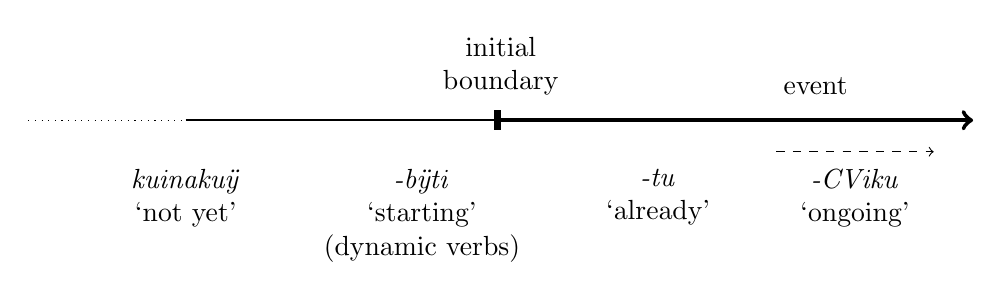
\begin{tikzpicture}
\draw[dotted] (-2,0)--(0,0);\draw [thick] [-|||]  (0,0) -- (4,0); \draw[ultra thick] [->]  (4,0) -- (10,0);
\draw[dashed][->] (7.5,-.4)--(9.5,-.4);
\node[align=center, above] at (4.0, .2){initial\\ boundary};%
\node[align=right, above] at (8.0, .2){event};%

\node[align=center, below] at (0.0,-.5)%
    {\textit{kuinakuÿ}\\‘not yet’};
\node[align=center, below] at (3.0,-.5)%
    {\textit{-bÿti}\\‘starting’\\(dynamic verbs)};
\node[align=center, below] at (6.0, -.5)%
    {\textit{-tu}\\‘already’ };
\node[align=center, below] at (8.5, -.5)%
    {\textit{-CViku}\\‘ongoing’ };
\end{tikzpicture}
\caption{Aspect markers acting on initial event boundaries}
\label{fig:AspectInitialBoundaries}
\end{figure}

\begin{figure}[!ht]

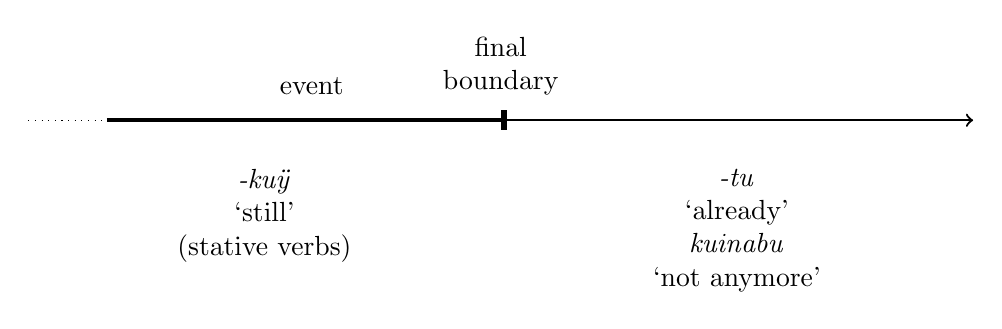
\begin{tikzpicture}
\draw[dotted] (-2,0)--(1,0);\draw [ultra thick] (-1,0) -- (4,0); \draw[thick] [|||->]  (4,0) -- (10,0);
\node[align=left, above] at (1.6, .2){event};%
\node[align=center, above] at (4.0, .2){final\\ boundary};%
\node[align=center, below] at (1.0,-.5)%
    {\textit{-kuÿ}\\‘still’\\(stative verbs)};

\node[align=center, below] at (7.0, -.5)%
    {\textit{-tu}\\‘already’\\\textit{kuinabu}\\‘not anymore’ };
\end{tikzpicture}
\caption{Aspect markers acting on final event boundaries}
\label{fig:AspectFinalBoundaries}
\end{figure}
\is{telicity|)}
\is{aktionsart|)}


\subsubsection{Iamitive perfect}\label{sec:Iamitive}\is{iamitive|(}

The most frequent of the tense and aspect markers of Paunaka is the omnipresent iamitive marker \textit{-tu}. The term “iamitive” is related to the better-known perfect. According to \citet[4]{Olsson2013}, iamitive markers are “aspectotemporal markers that seemingy [sic!] overlap with both the perfect and ‘already’”. Thus, a sentence like (\ref{ex:new23-dead}) can have various translations into English depending on the context.

\ea\label{ex:new23-dead}
\begingl
\glpreamble tipakutu\\
\gla ti-paku-tu\\
\glb 3i-die-\textsc{iam}\\
\glft ‘she is dead (already/now)’ \\or: ‘she has died (already/now)’
\endgl
%\trailingcitation{[]}
\xe

In his thesis, \citet[]{Olsson2013} described iamitives in some Southeast Asian languages in detail. Subsequently, \citet[]{DahlWalchli2016} proposed that the iamitive is a distinct gram type in a larger grammatical space that also includes perfects in the traditional sense and many other gram types that overlap in their uses. A new gram type, though with the name “new situation”, was also proposed by \citet[]{Ebert2001}, in analysing iamitive-like markers in Kiranti languages (reflected by the optional addition of “now” in the translation of (\ref{ex:new23-dead})).

Others have argued against gram status of the iamitive. Among them is \citet[]{Krajinovic2019}, who states that the differences from “traditional” perfects can still be explained within the functional realm of the perfect if we acknowledge that the perfect has distinct peculiarities in tenseless languages.\footnote{Actually, she identifies as a defining feature of perfects that they place the time the assertion is about (TT) posterior to the time the event took place (TSit) \citep[107]{Krajinovic2019}. However, this is not true for the Paunaka iamitive marker, which can also express that an event is currently ongoing.} I am agnostic as to the question whether the iamitive is a distinct gram type or should better be defined as a peculiar expression of the perfect gram or even be dismissed at all and be replaced by a more encompassing definition of perfect. I simply use the term “iamitive” here because the characteristics of the Paunaka marker fit relatively well the description of iamitive given by \citet[]{Olsson2013}. 

The iamitive is generally optional in Paunaka, in the sense that it does not enter into any obligatory binary distinction iamitive vs. non-iamitive, though its use is highly favoured in some situations. This should be kept in mind, when reading the following lines. 

According to \citet[4]{Olsson2013}, iamitives share with perfects the property of marking “the current relevance of a previous event”, but they differ from perfects in how they interact with the \isi{aktionsart} of a verb. This becomes apparent when considering stative verbs,\is{stative verb|(} since “certain types of states are particularly likely to be marked by iamitives, notably states that are the outcome of some natural process, such as ‘be ripe’ or ‘be grown up’” \citep[4]{Olsson2013}. Such states result from a “unidirectional development” of a “natural course of events” \citep[30]{Olsson2013}. This is exactly what we find in Paunaka. On stative predicates, the iamitive marker \textit{-tu} expresses, first, that the state holds at reference time, and second, that it is the result of some previous change,\is{resultative} i.e. that there existed a time prior to reference time in which the state did not hold. This is the main difference between an iamitive and a perfect, since the perfect does not imply that the state encoded by a stative verb currently holds \citep[cf.][9]{Olsson2013}.

The iamitive marker is \textit{-tu} in Paunaka and it is certainly related to the adverb \textit{metu} ‘ready, already’.

(\ref{ex:ripe-hair}) provides an example of a iamitive marker on a stative verb that encodes the result of a prior change of state, i.e. the hair colour of an elderly man, which has changed from black to grey or white, with the latter being expressed by the verb \textit{-yu} ‘be ripe’ in Paunaka. The example was elicited from Isidro.

\ea\label{ex:ripe-hair}
\begingl 
\glpreamble tiyutu nimukiji\\
\gla ti-yu-tu ni-muki-ji\\ 
\glb 3i-be.ripe-\textsc{iam} 1\textsc{sg}-hair-\textsc{col}\\ 
\glft ‘my hair is already white’\\ 
\endgl
\trailingcitation{[mdx-c120416ls.150]}%semi-elicitated
\xe

In the same situation, Miguel proposed an answer containing the stative verb for ‘white, clear’, see (\ref{ex:white-hair}). However, this is not the way the colour of elderly people’s hair is usually referred to in Paunaka. All the same, the iamitive marker equally attaches to the verb here.

\ea\label{ex:white-hair}
\begingl
\glpreamble pisururutu\\
\gla pi-sururu-tu\\
\glb 2\textsc{sg}-be.clear-\textsc{iam}\\
\glft ‘you are already white’
\endgl
\trailingcitation{[mdx-c120416ls.143]}
\xe


(\ref{ex:nat-proc-yes-tu}) is about a ripe fruit and also builds on the verb \textit{-yu} ‘be ripe’. As in (\ref{ex:white-hair}) above, the iamitive marker is used on the verb. It also attaches to \textit{kana} ‘this size’, which is a \isi{demonstrative adjective} and thus we have an example of non-verbal predication here. The adjective is always accompanied by a gesture showing the actual size. The sentence comes from a correction session with María S. (it slightly differed from the one she had originally produced).

\ea\label{ex:nat-proc-yes-tu}
\begingl
\glpreamble kanainatu chÿi te tayutu binikatu\\
\gla kana-ina-tu chÿi te ti-a-yu-tu bi-nika-tu\\
\glb this.size-\textsc{irr.nv}-\textsc{iam} fruit \textsc{seq} 3i-\textsc{irr}-be.ripe-\textsc{iam} 1\textsc{pl}-eat.\textsc{irr}-\textsc{iam}\\
\glft ‘once the fruit has this size, then it is ripe and then we can eat it’
\endgl
\trailingcitation{[rxx-e121128s-3.11]}
\xe

Although it is highly common to attach a iamitive marker to a stative predicate that can be analysed as encoding the result of a process, this is not obligatory. In the following example, no iamitive is used on the verb \textit{-yu} ‘be ripe’, possibly because the change of state is backgrounded here, the more important information being the actual state of being ripe as a precondition for the chicken eating the fruit. %It is thus excluded that the stative verb \textit{-yu} ‘be ripe’ is not a stative verb at all but an inchoative verb.
The sentence comes from María S., too.

\ea\label{ex:nat-proc-no-tu}
\begingl 
\glpreamble kuina chinijanea, kuina, abÿrÿsÿi si kue tayu chinijanea\\
\gla kuina chi-ni-jane-a kuina abÿrÿsÿi si kue ti-a-yu chi-ni-jane-a\\ 
\glb \textsc{neg} 3-eat-\textsc{distr}-\textsc{irr} \textsc{neg} guava yes if 3i-\textsc{irr}-be.ripe 3-eat-\textsc{distr}-\textsc{irr}\\ 
\glft ‘they (the chicken) don’t eat it, no, guavas, yes, they eat if they are ripe’\\ 
\endgl
\trailingcitation{[rxx-e121126s-3.36]}
\xe

If the stative verb does not encode the endpoint of a natural development per se, then such a reading is added by the iamitive marker.\is{stative verb|)}  It can, for example, combine with the non-verbal existential \isi{copula} \textit{kaku}, and in this case, it expresses that something has come into existence by reference time that has not been there before. This can be seen in the following example (\ref{ex:ticks}).

The context is as follows: Miguel and I had paid José a visit and when we came back to the village, we were bitten by some small ticks. Miguel made a comment that there were many ticks, and María S. reacted with a question, which can rather be read as an expression of surprise than as a request for information. Apparently, she was surprised that the tick season had already started, since she had not noticed any ticks up to this point.

\ea\label{ex:ticks}
\begingl 
\glpreamble ¿kakutu samuchu?\\
\gla kaku-tu samuchu\\ 
\glb exist-\textsc{iam} tick.sp\\ 
\glft ‘there are ticks already?’\\ 
\endgl
\trailingcitation{[mrx-c120509l.149]}
\xe

Another case in which the iamitive adds a development reading to a stative predicate, but this time a verbal one, is (\ref{ex:know-cos}). Together with the iamitive marker, the verb \textit{-(i)chuna} ‘know, be capable, be able’ encodes that knowledge has been acquired by learning. However, the focus still lies on the state after the process of learning and not on the process itself.

In this example, Juana talks about her grandson.

\ea\label{ex:know-cos}
\begingl 
\glpreamble tijÿku i netuku xhikuera i tichunatu te i tiyunu kuarterayae...\\
\gla ti-jÿku i nÿ-etuku xhikuera i ti-ichuna-tu te i ti-yunu kuartera-yae\\ 
\glb 3i-grow and 1\textsc{sg}-put school and 3i-be.capable-\textsc{iam} \textsc{seq} and 3i-go military.base-\textsc{loc}\\ 
\glft ‘he grew and I put him into school and once he had acquired knowledge (i.e. learned), then he went to the military base...’\\ 
\endgl
\trailingcitation{[jxx-p110923l-1.173-176]}
\xe

Finally, the iamitive also appears on nouns denoting high age, when they are used as a predicate,\is{nominal predicate} but not if they are an argument of the clause. Compare (\ref{ex:old-woman-2}), where \textit{juberÿpu\-nÿtu} ‘I am an old woman’ is the predicate, with (\ref{ex:old-woman-1}), in which \textit{juberÿpu\-mÿnÿ} ‘dear old woman’ is the object of the clause and thus bears no iamitive marker.


(\ref{ex:old-woman-2}) is a statement by María C. about herself.

\ea\label{ex:old-woman-2}
\begingl 
\glpreamble juberÿpunÿtu kuina puero trabakuinabu\\
\gla juberÿpu-nÿ-tu kuina puero trabaku-ina-bu\\ 
\glb old.woman-1\textsc{sg}-\textsc{iam} \textsc{neg} can work-\textsc{irr.nv}-\textsc{dsc}\\ 
\glft ‘I am old, I cannot work anymore’\\ 
\endgl
\trailingcitation{[uxx-p110825l.203]}
\xe

In (\ref{ex:old-woman-1}), Juana talks about the chance she once had to go to Europe to work there. In the end, she did not go; this is why the frustrative is used here.

\ea\label{ex:old-woman-1}
\begingl 
\glpreamble niyunaini nichenenaikupa juberÿpumÿnÿ\\
\gla ni-yuna-ini ni-chenenaiku-pa juberÿpu-mÿnÿ\\ 
\glb 1\textsc{sg}-go.\textsc{irr}-\textsc{frust} 1\textsc{sg}-care.for-\textsc{dloc.irr} old.woman-\textsc{dim}\\ 
\glft ‘I would have gone (to Austria) to care for an old woman’\\ 
\endgl
\trailingcitation{[jxx-e120516l-1.015]}
\xe


Considering dynamic verbs, we can distinguish between telic and atelic\is{telicity|(} predicates.\is{aktionsart|(} \citet[19]{Olsson2013} predicts that “[w]ith a telic predicate, the ‘new situation’ asserted by the iamitive corresponds to the situation following the final boundary (or, with an achievement, following the only boundary)”. In combination with atelic verbs, however, the action can either be finished or ongoing. This is because “a iamitive can be interpreted as applying either to the initial boundary, thus yielding an on-going interpretation, or to the final boundary, yielding a completed, ‘past’ interpretation” \citep[19]{Olsson2013}. 

Let us first consider some telic verbs. First of all, the iamitive marker can encode a state resulting from an event as in (\ref{ex:die-iam}).\is{resultative}

The sentence comes from Juana telling the story about the fox and the jaguar. At this point of the story, the jaguar has been dead for several months already, and the fox comes back to the pond where he died to spitefully speak with his skeleton. The fox starts in Spanish, but continues the sentence in Paunaka.\footnote{The Spanish phrase \textit{¿no ve?} is not to be understood literally (‘he/she doesn’t see’). In Bolivia, it is used as a tag question to seek confirmation similar to English ‘right?’ or ‘you know?’ \citep[45]{Mendoza2015}.}

\ea\label{ex:die-iam}
\begingl
\glpreamble “¿no ve? tío, ¡pipakutu!”\\
\gla {no ve} tío pi-paku-tu\\
\glb {right} uncle 2\textsc{sg}-die-\textsc{iam}\\
\glft ‘“right, uncle? you’re dead!”’
\endgl
\trailingcitation{[jmx-n120429ls-x5.286-287]}
\xe

The fact that there is a state resulting from a punctual event is not enough to trigger iamitive marking, though. There is a complex interplay between aktionsart\is{aktionsart|)} of the verb, \isi{reality status}, derivational morphology and also middle voice\is{middle voice|(}. Middle verbs often imply a continuous state, and thus \textit{-tupunu-bu} ‘arrive’ already implies a \isi{resultative} state as opposed to the punctual \textit{-tupunu} ‘reach’; see (\ref{ex:arrive-no-iam}), where we need a perfect in the English translation, but no iamitive in the original Paunaka sentence. The same is true for the middle verb \textit{-yÿtiku-bu} ‘cook’, which relates to \textit{-yÿtiku} ‘set (a pot) on fire’ and for all posture verbs.

(\ref{ex:arrive-no-iam}) was elicited from María S.

\ea\label{ex:arrive-no-iam}
\begingl
\glpreamble chuinepaiku titupunubu nichechapÿi\\
\gla uchuine-paiku ti-tupunubu ni-chechapÿi\\
\glb just.now-\textsc{punct} 3i-arrive 1\textsc{sg}-son \\
\glft ‘my son has just arrived’
\endgl
\trailingcitation{[rxx-e181022le.124]}
\xe
\is{middle voice|)}

If \textit{-tupunubu} ‘arrive’ is combined with a iamitive, it rather evokes anteriority or earliness readings or it expresses that an expectation is fulfilled, which is just what we expect from a iamitive \citep[cf.][21]{Olsson2013}. Prior to (\ref{ex:arrive-iam}), María S. had told me that Federico and Swintha had already informed her that I would come to Bolivia.

\ea\label{ex:arrive-iam}
\begingl
\glpreamble jaa metu pitupunubutu naka\\
\gla jaa metu pi-tupunubu-tu naka\\
\glb \textsc{afm} already 2\textsc{sg}-arrive-\textsc{iam} here\\
\glft ‘yes, and now you have arrived here’
\endgl
\trailingcitation{[rxx-e181017l.005]}
\xe

In (\ref{ex:arrive-iam}), the iamitive combines with the adverb \textit{metu} ‘already, ready’ to indicate current relevance. In (\ref{ex:broken-iam}) on the other hand, \textit{metu} and the iamitive-marked verb indicate earliness of a resultative state. The example was elicited from María S. and corresponds to an invented situation, in which a mother asks her daughter who may have broken a pot, and the daughter answers that she doesn’t know and that the pot was already broken, when she saw it. Note that the iamitive marker also occurs on the first atelic verb \textit{-imu} ‘see’ here.

\ea\label{ex:broken-iam}
\begingl
\glpreamble nimutu metu terabajikutu\\
\gla ni-imu-tu metu ti-rabajiku-tu\\
\glb 1\textsc{sg}-see-\textsc{iam} already 3i-break-\textsc{iam}\\
\glft ‘when I saw it, it was already broken’
\endgl
\trailingcitation{[rxx-e181021les.222]}
\xe

Current relevance is also at work in (\ref{ex:stuck}), where use of the iamitive indicates that the result of the dog’s sticking its head into the glass (or pot) is of importance. The example comes from Miguel telling José the \isi{frog story}. The fact that the dog’s head got stuck was expressed lexically in the sentence that followed. 

\ea\label{ex:stuck}
\begingl
\glpreamble i naka chipurutukutu eka kabe chichÿti naka eka tachukÿyae\\
\gla i naka chi-purutuku-tu eka kabe chi-chÿti naka eka tachu-kÿ-yae\\
\glb and here 3-put.in-\textsc{iam} \textsc{dem}a dog 3-head here \textsc{dem}a small.pot-\textsc{clf}:bounded-\textsc{loc}\\
\glft ‘and here the dog has stuck his head into the small pot here’
\endgl
\trailingcitation{[mox-a110920l-2.052]}
\xe

So far, we have only looked at telic verbs with \isi{realis} RS. It is also possible to combine an \isi{irrealis} verb with iamitive. Irrealis, among other things, can express \isi{future reference} of an event. Combination with the iamitive can then indicate that the final boundary has not yet been reached although the measures have been taken to reach it. This is the case in (\ref{ex:breed-iam}), where the final boundary is the hatching of the chicken. The sentence was elicited from Juana, who had just told me that her hen was breeding.

\ea\label{ex:breed-iam}
\begingl
\glpreamble tipuichakatu takÿrajanemÿnÿ\\
\gla ti-puichaka-tu takÿra-jane-mÿnÿ\\
\glb 3i-hatch.\textsc{irr}-\textsc{iam} chicken-\textsc{distr}-\textsc{dim}\\
\glft ‘it will hatch eggs (lit.: little chicken)’
\endgl
\trailingcitation{[jxx-e110923l-2.086]}
\xe

Atelic\is{aktionsart|(} verbs with a iamitive marker can be interpreted as encoding either an ongoing or a completed action as is predicted by \citet[19]{Olsson2013}, because the iamitive can apply to either the initial or the final boundary of the event. Thus in an invented situation, in which a mother invites her son to eat something, the answer including the iamitive can either mean that the son has already eaten or that he is eating at that very moment (and the mother does not see him because he is sitting behind the house), see (\ref{ex:atelic-iam}). 

\ea\label{ex:atelic-iam}
\begingl
\glpreamble nÿnikutu\\
\gla nÿ-niku-tu\\
\glb 1\textsc{sg}-eat-\textsc{iam}\\
\glft ‘I am already eating’\\ or: ‘I have eaten already’
\endgl
\trailingcitation{[rxx-e181021les.202, 205]}
\xe
\is{aktionsart|)}

Equally, if the mother asks her son to send her daughter to go and fetch water, the answer including the iamitive can either indicate that the daughter has completed the task or is busy on the task at that very moment, as in (\ref{ex:atelic-iam-2}), which was also elicited from María S.

\ea\label{ex:atelic-iam-2}
\begingl
\glpreamble tiyunutu tepa ÿne\\
\gla ti-yunu-tu ti-epa ÿne\\
\glb 3i-go-\textsc{iam} 3i-take.\textsc{irr} water\\
\glft ‘she is already going to fetch water’\\or: ‘she already went to fetch water’
\endgl
\trailingcitation{[rxx-e181022le]}
\xe
\is{telicity|)}

However, if it is necessary to clarify that the action is taking place right now, speakers can also resort to continuous\is{continuous|(} marking (see \sectref{sec:ActiveVerbs_RDPL}). They can then add the iamitive to the continuous verb. Additionally, an adverb can help to clarify temporal reference. Both strategies are combined in (\ref{ex:atelic-cont-iam}), which was elicited from Juana, providing her with the same invented context as María S. in (\ref{ex:atelic-iam}) above.

\ea\label{ex:atelic-cont-iam}
\begingl
\glpreamble ¡ninikutu mimi! ninikukuikutu tanÿma naka\\
\gla ni-niku-tu mimi ni-niku-kuiku-tu tanÿma naka\\
\glb 1\textsc{sg}-eat-\textsc{iam} mum 1\textsc{sg}-eat-\textsc{cont}-\textsc{iam} now here\\
\glft ‘I am already eating, mum! I am already eating here right now’
\endgl
\trailingcitation{[jxx-e181104l-3]}
\xe
\is{continuous|)}

The following two examples were produced more spontaneously, and we can notice that the iamitive marker on one and the same verb, \textit{-kutijiku} ‘escape, flee’, can express that the action, i.e. the escape, is successfully completed as in (\ref{ex:iam-flee-1}), or ongoing as in (\ref{ex:iam-flee-2}).

In (\ref{ex:iam-flee-1}), Juana tells me about a criminal in-law of hers who had hidden away in the woods. When he was detected, some people went to the woods in search of him, but he had managed to escape before.

\ea\label{ex:iam-flee-1}
\begingl
\glpreamble kuina kakuinabu nauku kimenubu, tikutijikutu\\
\gla kuina kaku-ina-bu nauku kimenu-bu ti-kutijiku-tu\\
\glb \textsc{neg} exist-\textsc{irr.nv}-\textsc{dsc} there woods-\textsc{dsc} 3i-flee-\textsc{iam}\\
\glft ‘he wasn’t there anymore in the woods, he had escaped’
\endgl
\trailingcitation{[jxx-p120430l-2.053]}
\xe

(\ref{ex:iam-flee-2}) refers to the picture in the \isi{frog story} in which the dog is running away from the bees. Its escape is thus ongoing. The example comes from Miguel.

\ea\label{ex:iam-flee-2}
\begingl
\glpreamble chijikiu eka kabe tikutijikutu i eka janejane cheikukuiku\\
\gla chijikiu eka kabe ti-kutijiku-tu i eka jane-jane chÿ-eikukuiku\\
\glb however \textsc{dem}a dog 3i-flee-\textsc{iam} and \textsc{dem}a wasp-\textsc{distr} 3-chase\\
\glft ‘nonetheless, the dog is fleeing and the wasps are chasing it’
\endgl
\trailingcitation{[mox-a110920l-2.104]}
\xe

Two more examples with telic verbs follow. In (\ref{ex:iam-atel-1}) by Miguel, the initial boundary of the action is triggered (or established) by the iamitive. The sentence provides the funny climax of one of the episodes of the story of the fox and the jaguar. The jaguar has caught a vulture and wants to eat him, and the vulture seemingly surrenders and proposes that the jaguar plucks him except for his wings and throws him up into the air so that he would fall down back into his open mouth. The jaguar obeys, but instead of falling, the vulture defecates into the jaguar’s mouth and then flies away. It is thus the initial boundary of flying, the take-off, that is important in (\ref{ex:iam-atel-1}).

\ea\label{ex:iam-atel-1}
\begingl
\glpreamble i te tibÿbÿkutuji echÿu sÿmÿ tiyunu\\
\gla i te ti-bÿbÿku-tu-ji echÿu sÿmÿ ti-yunu\\
\glb and \textsc{seq} 3i-fly-\textsc{iam}-\textsc{rprt} \textsc{dem}a vulture 3i-go\\
\glft ‘and then the vulture flew off, it is said, and went (i.e. escaped)’
\endgl
\trailingcitation{[jmx-n120429ls-x5.211]}
\xe

In (\ref{ex:iam-atel-3}), the atelic verb\is{telicity} \textit{-pajÿku} ‘stay’ is turned into a non-reversed or even irreversible state (‘have stayed ever since, stay for good’) by addition of the iamitive. The example also comes from the story of the fox and the jaguar, but this time is narrated by María S. on another occasion. It is the jaguar who – tricked by the fox – jumps into the water and drowns. 

\ea\label{ex:iam-atel-3}
\begingl
\glpreamble tijipaikuji ÿneji te tepajÿkutu ÿneyae\\
\gla ti-jipaiku-ji ÿne-ji te ti-pajÿku-tu ÿne-yae\\
\glb 3i-jump.down-\textsc{rprt} water-\textsc{rprt} \textsc{seq} 3i-stay-\textsc{iam} water-\textsc{loc}\\
\glft ‘he jumped into the water and then he stayed in the water for good, it is said’
\endgl
\trailingcitation{[rxx-n120511l-1.039]}
\xe


(\ref{ex:iam-flee-1})--(\ref{ex:iam-atel-3}) all consist of two combined clauses,\is{complex sentence|(} but the iamitive is only marked once – an exception possibly being (\ref{ex:iam-flee-1}), whose first clause is marked for discontinuous, a category related to the iamitive, see \sectref{sec:Discontinuous} below. \citet[39]{Olsson2013} found that in clause combining, iamitives are often used to indicate temporal sequentiality. In all the examples he gives in his work, the iamitive appears in a clause that expresses the temporally anterior event. As for Paunaka, there are some examples that seem to verify this analysis, while others contradict it. Consider (\ref{ex:predicate1}) and (\ref{ex:predicate2-te}). In the first of them, the first event in the sequence is marked, in the second one it is the second event that receives iamitive aspect. 
Note that both clauses have irrealis RS for different reasons: (\ref{ex:predicate1}) is from a general description of how to use a clay pot, while (\ref{ex:predicate2-te}) has a habitual past reading. Both sentences are about usage of a clay pot and both come from Juana.

\ea\label{ex:predicate1}
\begingl 
\glpreamble tibururukatu ÿne i pijuka\\
\gla ti-bururuka-tu ÿne i pi-juka\\ 
\glb 3i-boil.\textsc{irr}-\textsc{iam} water and 2\textsc{sg}-pour.solid.\textsc{irr}\\ 
\glft ‘the water boils (now) and you pour it (i.e. the food) in’\\ 
\endgl
\trailingcitation{[jxx-d110923l-3]}
\xe

\ea\label{ex:predicate2-te}
\begingl 
\glpreamble taima te binikatu\\
\gla ti-a-ima te bi-nika-tu\\ 
\glb 3i-\textsc{irr}-be.cooked \textsc{seq} 1\textsc{pl}-eat.\textsc{irr}-\textsc{iam}\\ 
\glft ‘when it was done, then we would/could eat it (i.e. the food)’\\ 
\endgl
\trailingcitation{[jxx-d110923l-2.25]}
\xe

In both examples above, the iamitive could have probably also been attached to the other clause instead or additionally. Recall that \citet[]{Ebert2001} speaks of importance of a new situation, and \citet[9]{Olsson2013} notes that iamitives are often translated with “now”. Just like the English word “now” could mark either of the two events in (\ref{ex:predicate1}) and (\ref{ex:predicate2-te}) (ignoring for a moment the fact that “now” is not compatible with habitual contexts at all), the iamitive is possible on both predicates. This is because being optional the iamitive does not encode any absolute properties of the event’s tempo-aspectual setting, but simply signals what the speaker finds worth being marked as the new situation. In (\ref{ex:predicate1}), the iamitive is encodes that event 1 has to be realised in order for event 2 to be possible or appropriate. In (\ref{ex:predicate2-te}), however, the function of the iamitive is to close the statement \citep[cf.][8]{Olsson2013}. The use of the iamitive thus signals that the discourse topic is completed and we can expect a switch to another topic or another (discourse) aspect of the topic. We often find an iamitive on the last predicate of a chain of clauses which all provide information to the same overarching discourse topic.\is{complex sentence|)} 

(\ref{ex:predicate2}) provides another example of the use of \textit{-tu} in a clause that closes the description of a sequence of events. It was produced by Juana, after she had found loam for her clay pot in order to give us a description of what she would do now. Following the sentence in (\ref{ex:predicate2}), she talked about bringing the loam to her house and resume the production of the pot there, so there is a change of location, a new, separate step in the development of her pot, anticipated by the use of the iamitive here.

\ea\label{ex:predicate2}
\begingl 
\glpreamble betuku naka bichÿtiyae i biyunatu\\
\gla bi-etuku naka bi-chÿti-yae i bi-yuna-tu\\ 
\glb 1\textsc{pl}-put here 1\textsc{pl}-head-\textsc{loc} and 1\textsc{pl}-go.\textsc{irr}-\textsc{iam}\\ 
\glft ‘we put it (the bag) here on our head and we can go (now)’\\ 
\endgl
\trailingcitation{[jmx-d110918ls-2.02-03]}
\xe

It should have become clear by now that the iamitive has a wide range of different functions, and since it is so multifunctional, it is no surprise that it is used very frequently. We often find the iamitive on states that result\is{resultative} from a previous unidirectional development, we find it with completed and ongoing actions, and we find it in clause combining,\is{complex sentence} often together with the \isi{sequential} \isi{connective} \textit{te} ‘then’ and with the adverb \textit{metu} ‘already, ready’ as well as borrowed forms of the Spanish adverb \textit{después} ‘after’ (borrowed as e.g. \textit{depue}, \textit{repue}). However, there is one context in which we do not find the iamitive: \isi{negation}.\footnote{There are a handful of examples in the corpus in which the iamitive is found in a negative clause, but they are so few that they should probably be treated as mistakes.} 

Cross-linguistically, iamitives often combine with negation and then they usually exhibit either a discontinuative meaning or a meaning described as ‘not yet/still not’ \citep[cf.][35--36]{Olsson2013}. Paunaka  has separate aspect markers for the \isi{discontinuous} and the \isi{incompletive} (the latter being the term chosen here for the meaning of ‘not yet’ and its positive counterpart ‘still’). The iamitive marker is usually not found in negative clauses\is{negation} with one exception: If the \isi{negative particle} \textit{kuina} is the predicate itself, \textit{-tu} can be added after the \isi{discontinuous} marker to emphasise that the negative state that is contrasted to the anterior positive state holds at reference time, see (\ref{ex:kuinabutu}). The sentence comes from María S. telling the story about the two hunters and the devil. This is what one of the men tells the devil after the latter has eaten up everything the two men had hunted.

 \ea\label{ex:kuinabutu}
\begingl
\glpreamble “kuinabutu chija nenikapi”\\
\gla kuina-bu-tu chija nÿ-nika-pi\\
\glb \textsc{neg}-\textsc{dsc} what 1\textsc{sg}-feed.\textsc{irr}-2\textsc{sg}\\
\glft ‘“there isn’t anything left that I could give you to eat”’
\endgl
\trailingcitation{[rxx-n120511l-2.45-46]}
\xe

The following sections provide information about aspects related to the iamitive, discontinuous aspect is described in \sectref{sec:Discontinuous} and incompletive aspect in \sectref{sec:Incompletive}.\is{iamitive|)} 


\subsubsection{Discontinuous}\label{sec:Discontinuous}\is{discontinuous|(}
\is{negation|(}
The discontinuous marker \textit{-bu} is exclusively used in negative clauses and can be translated with ‘anymore’. It expresses that a state does not hold any longer or that an action is not performed anymore. It thus targets a final boundary, but unlike the English adverb, it seems to imply the state after the final boundary most of the times rather than focus on the final boundary itself, so \textit{kuina x-bu} means ‘after x, be in a state of not-x’ rather than ‘x is over (thus y)’. To demonstrate this, consider the following English sentences, which all include the adverb \textit{anymore}.

\begin{enumerate}
\item He does not eat anymore (because he is ill).\label{item:dsc-1}
\item He won’t eat anymore today (because he has eaten so much).\label{item:dsc-2}
\item He  isn’t eating anymore (so you can talk to him now).\label{item:dsc-3}
\end{enumerate}

The discontinuous marker predominantly occurs in contexts similar to \ref{item:dsc-1}. (state ‘no-x after x’ has a long duration or is persistent), and contexts like \ref{item:dsc-2}. (state ‘no-x after x’ has a limited duration) have also been found. However, as for \ref{item:dsc-3}. (state ‘no-x’ corresponds to end of x), there are only very few examples that could be analysed as corresponding to similar contexts. 
 
The discontinuous marker can either attach to the predicate or to the negative particle or to both with no apparent difference in meaning. Consider (\ref{ex:DSCnew-1}). There are two juxtaposed clauses: in the first one the marker attaches to the verb and in the second one to the negative particle. It comes from Juana who was talking about the making of the reservoir in Santa Rita. Once it was ready, people from Santa Rita did not have to walk far anymore to get water.

\ea\label{ex:DSCnew-1}
\begingl
\glpreamble kuina biyunabu Naranjito, kuinabu biyuna naka Tavistayae\\
\gla kuina bi-yuna-bu Naranjito kuina-bu bi-yuna naka Tavista-yae\\
\glb \textsc{neg} 1\textsc{pl}-go.\textsc{irr}-\textsc{dsc} Naranjito \textsc{neg}-\textsc{dsc} 1\textsc{pl}-go.\textsc{irr} here Altavista-\textsc{loc}\\
\glft ‘we don’t have to go to Naranjito anymore, we don’t have to go to \isi{Altavista} anymore’
\endgl
\trailingcitation{[jxx-p120515l-2.207-208]}
\xe

An example in which \textit{-bu} attaches to both negative particle and predicate is (\ref{ex:dsc-1}). It is a statement by María C. about her ability to see, which has decreased over time, since she is an old lady.

\ea\label{ex:dsc-1}
\begingl 
\glpreamble kuinabu naimubÿkebu\\
\gla kuina-bu nÿ-a-imubÿke-bu\\ 
\glb \textsc{neg}-\textsc{dsc} 1\textsc{sg}-\textsc{irr}-see.well-\textsc{dsc}\\ 
\glft ‘I can’t see well anymore’\\ 
\endgl
\trailingcitation{[uxx-p110825l.013]}
\xe

%In negative existential sentences, there is often no separate predicate to which the discontinuous marker could attach, the negative particle being the predicate itself. This is the case in: kakukuÿnube echÿu paunakanube o kuinabunubetu, ump-p110815sf.127

Although the discontinuous marker and the middle marker\is{middle voice} are homophonous, they cannot be confused. The middle marker has an allophone \textit{-pu} that occurs after \isi{irrealis}. The predicates to which the discontinuous marker attaches necessarily have \isi{irrealis} RS, since they are all negated, and the form of the discontinuous marker is always \textit{-bu}. An example in which both markers co-occur has already been given in \sectref{sec:Middle_voice} (ex. (\ref{ex:MID-DSC})).

A few more examples of the discontinuous marker shall be given here.

(\ref{ex:dsc-3}) was produced by Juana, when I was visiting her in Santa Cruz, where she was living at that time. She uttered the assumption that I would not go back to Concepción from Santa Cruz, but rather stay there in order to leave for Germany directly (which was not the case, since I had indeed planned to spend a few more days in Concepción before coming back to Santa Cruz and subsequently travel back to Germany).

\ea\label{ex:dsc-3}
\begingl 
\glpreamble kuina piyunupunabu Concecionyae\\
\gla kuina pi-yunupuna-bu Concecion-yae\\ 
\glb \textsc{neg} 2\textsc{sg}-go.back.\textsc{irr}-\textsc{dsc} Concepción-\textsc{loc}\\ 
\glft ‘you won’t go back to Concepción anymore’\\ 
\endgl
\trailingcitation{[jxx-p120430l-1.134]}
\xe

%In (\ref{ex:dsc-4}) the discontinuous marker is found on a non-verbal predicate.\footnote{Note that verbs from Spanish are often borrowed as non-verbal predicates, see \sectref{sec:borrowed_verbs}.} The sentence is from the account of the Paunaka history given by Miguel and presents the reason why the first inhabitant of Santa Rita was allowed to move away from Altavista to found a new village.
%
%\ea\label{ex:dsc-4}
%\begingl 
%\glpreamble kuina pueroinabu trabakuinabu chitÿpi echÿu patron\\
%\gla kuina puero-ina-bu trabaku-ina-bu chi-tÿpi echÿu patron\\ 
%\glb \textsc{neg} can-\textsc{irr.nv}-\textsc{dsc} work-\textsc{irr.nv}-\textsc{dsc} 3-\textsc{ben} \textsc{dem}b boss\\ 
%\glft ‘he couldn’t work for the \textit{patrón} anymore’\\ 
%\endgl
%\trailingcitation{[mxx-p110825l.024-025]}
%\xe

(\ref{ex:DSCnew-4}) has a nominal predicate. Miguel speaks of a village close to Santa Rita which was abandoned.

\ea\label{ex:DSCnew-4}
\begingl
\glpreamble kuinabutu jentenubeinabu nauku\\
\gla kuina-bu-tu jente-nube-ina-bu nauku\\
\glb \textsc{neg}-\textsc{dsc}-\textsc{iam} man-\textsc{pl}-\textsc{irr.nv}-\textsc{dsc} there\\
\glft ‘there are no people anymore there now’
\endgl
\trailingcitation{[mty-p110906l.134]}
\xe

(\ref{ex:DSCnew-1})–(\ref{ex:DSCnew-4}) above all refer to persistent states resulting from the termination of an event x. As has been stated in the introduction to this section, this is the most typical usage of the discontinuous marker. In the following two examples, however, \textit{-bu} is used to refer to easily reversible states or states of a limited duration.

In (\ref{ex:DSCnew-5}), Juana speaks about the weather after there was heavy rainfall the day before. Following this statement, she mentioned that the forecast had announced rainfall for the next day, so the state definitely has no long duration. Note that Juana uses the adverb \textit{metu} to encode exactly this short duration.

\ea\label{ex:DSCnew-5}
\begingl
\glpreamble pero metu kuina tikebabu\\
\gla pero metu kuina ti-keba-bu\\
\glb but already \textsc{neg} 3i-rain.\textsc{irr}-\textsc{dsc}\\
\glft ‘but for now it is not going to rain anymore’
\endgl
\trailingcitation{[jxx-e120516l-1.101]}
\xe


In (\ref{ex:dsc-5}), María C. is speaking about the scarceness of corn. As a consequence, she will soon not be able to drink chicha, a drink made from corn, but has to drink water. The state is reversible because as soon as she gets some money, María C. can buy more corn and make chicha again (i.e. the shortage is not due to crop failure in this case; due to her advanced age, the speaker did not have a field anymore at that time).

\ea\label{ex:dsc-5}
\begingl
\glpreamble kakumÿnÿ amukemÿnÿ te tibukapu echÿu te kuinabu nea aumue\\
\gla kaku-mÿnÿ amuke-mÿnÿ te ti-buka-pu echÿu te kuina-bu nÿ-ea aumue\\
\glb exist-\textsc{dim} corn-\textsc{dim} \textsc{seq} 3i-finish.\textsc{irr}-\textsc{mid} \textsc{dem}b \textsc{seq} \textsc{neg}-\textsc{dsc} 1\textsc{sg}-drink.\textsc{irr} chicha\\
\glft ‘there is little corn and when it is finished, then I cannot drink chicha anymore’
\endgl
\trailingcitation{[ump-p110815sf.693]}
\xe

Finally, the last two examples given here demonstrate a possible use of the marker that targets the end of an event rather than the state after it. One of them is (\ref{ex:DSCnew-3}), which was elicited from María S. providing her with the context that somebody is lying in a hammock.

\ea\label{ex:DSCnew-3}
\begingl
\glpreamble kuina timukabu\\
\gla kuina ti-muka-bu\\
\glb \textsc{neg} 3i-sleep.\textsc{irr}-\textsc{dsc}\\
\glft ‘she is not sleeping anymore’
\endgl
\trailingcitation{[rxx-e181024l]}
\xe

Another example that possibly targets the end of an event is (\ref{ex:DSCnew-2}), but it cannot be excluded that it refers to a reversible state after the event. The sentence was produced by María S. when some piglets had shown up at her yard grunting, but then suddenly got quiet because they started to suckle at their mother’s teats. Now, it is not clear whether María S. was referring to the stopping of grunting at that very moment or the fact that the piglets would stop grunting for a while, since they were not hungry anymore.

\ea\label{ex:DSCnew-2}
\begingl
\glpreamble tujijaneutu, nechikue kuina tasabaibujane\\
\gla ti-uji-jane-u-tu nechikue kuina ti-a-sabai-bu-jane\\
\glb 3i-suckle-\textsc{distr}-\textsc{real}-\textsc{iam} therefore \textsc{neg} 3i-\textsc{irr}-shout-\textsc{dsc}-\textsc{distr}\\
\glft ‘they are suckling now, thus they are not grunting anymore’\\or: ‘..., thus they do not grunt anymore’
\endgl
\trailingcitation{[rmx-e150922l.155-156]}
\xe
\is{negation|)}
\is{discontinuous|)}


\subsubsection{Incompletive}\label{sec:Incompletive}\is{incompletive|(}

Unlike the \isi{iamitive} (see \sectref{sec:Iamitive}) and the \isi{discontinuous} marker (see \sectref{sec:Discontinuous}), the incompletive marker \textit{-kuÿ} ‘still, (not) yet’ can occur in positive and in negative sentences. It marks an event as ongoing at reference time, while simultaneously implying the termination of the event at a later point in time.

In positive sentences, \textit{-kuÿ} is found on predicates denoting reversible states. It always has stative overtones, even if the verb is active\is{active verb}. It would not be used in a sentence corresponding to ‘He is still eating (you cannot talk to him right now)’, i.e. it is not compatible with a progressive interpretation of an action.

While the \isi{iamitive} is found on states that mark the outcome of a “natural course of events” \citep[30]{Olsson2013}, the incompletive is typically used with words denoting the starting point of such a development, usually nouns denoting young age, and sometimes also verbs that are used to illustrate young age, which means they are not understood actively but statively in these cases. In (\ref{ex:INCMPL-5}), we find the incompletive marker being attached to a noun, in (\ref{ex:INCMPL-4}) to an adjective, and in (\ref{ex:INCMPL-3}) to an adjective and to a verb.

(\ref{ex:INCMPL-5}) was produced by Miguel, when talking about the old days with Juan C. I do not know what exactly this sentence refers to, because I did not understand the previous sentences, but it has to do with the behaviour of \textit{karay} towards the people in Santa Rita.

\ea\label{ex:INCMPL-5}
\begingl 
\glpreamble i nÿti nikechu: “kuina pueroina, pue nÿti aitubuchepÿikuÿni”\\
\gla i nÿti ni-kechu kuina puero-ina pue nÿti aitubuchepÿi-kuÿ-ni\\ 
\glb and 1\textsc{sg.prn} 1\textsc{sg}-say \textsc{neg} can-\textsc{irr.nv} well 1\textsc{sg.prn} boy-\textsc{incmp}-1\textsc{sg}\\ 
\glft ‘and I said: “I can’t, I am still a young man”’\\ 
\endgl
\trailingcitation{[mqx-p110826l.386]}
\xe

In (\ref{ex:INCMPL-4}) the incompletive marker attaches to the \isi{demonstrative adjective} \textit{kana} ‘be of this size’. The sentence comes from María C. in telling about the hard childhood and youth she had.

\ea\label{ex:INCMPL-4}
\begingl
\glpreamble kanakuÿnemÿnÿni tepaku nÿa ja\\
\gla kana-kuÿ-ne-mÿnÿ-ni ti-paku nÿ-a ja\\
\glb this.size-\textsc{incmp}-1\textsc{sg}-\textsc{dim}-\textsc{deict} 3i-die 1\textsc{sg}-father \textsc{afm}\\
\glft ‘when I still was this size (showing with hands), my father died’
\endgl
\trailingcitation{[ump-p110815sf.149]}
\xe


If the incompletive marker combines with active verbs,\is{active verb|(} they normally express a state rather than an action. In (\ref{ex:INCMPL-3}), the marker is found on a nominal predicate first and then on an active verb; however, this does not mean that the action is going on at that very moment, but rather that the referents are in a state in which the action is still being carried out appropriately. It refers to some puppies that were running around in the yard of María S. and were apparently very hungry. Somebody had brought them to Santa Rita from Concepción, although they were still much too small to survive without being fed by their mother.

\ea\label{ex:INCMPL-3}
\begingl 
\glpreamble hmm, sepitÿkuÿjaneyu tujikukuÿjaneyu\\
\gla hmm sepitÿ-kuÿ-jane-yu ti-ujiku-kuÿ-jane-yu\\ 
\glb \textsc{intj} small-\textsc{incmp}-\textsc{distr}-\textsc{ints} 3i-suckle-\textsc{incmp}-\textsc{distr}-\textsc{ints}\\ 
\glft ‘hmm, they are still very small, they still suckle a lot’\\ 
\endgl
\trailingcitation{[rxx-e120511l.364]}
\xe


In (\ref{ex:still-alive}), the active verb \textit{-nÿnÿiku} has to be understood as ‘be alive’. It is contrasted with the current irreversible state of death, although this is not expressed lexically. The use of the adverb \textit{metu} ‘already, ready’ is interesting here. It is often used together with the iamitive, but seems to be compatible with stative incompletive readings of morphologically active verbs. The sentence comes from María S. and refers to her late mother who taught her how to weave.

\ea\label{ex:still-alive}
\begingl
\glpreamble timesumeikunÿbane nÿenu metu tenÿnÿikukuÿ\\
\gla ti-mesumeiku-nÿ-bane nÿ-enu metu ti-nÿnÿiku-kuÿ\\
\glb 3i-teach-1\textsc{sg}-\textsc{rem} 1\textsc{sg}-mother already 3i-live-\textsc{incmp}\\
\glft ‘my mother taught me long ago when she was still alive’
\endgl
\trailingcitation{[rxx-e181022le]}
\xe

A second example in which \textit{metu} is used in a similar fashion is (\ref{ex:still-fish}), which comes from Juana. It is a somehow incomplete sentence which she produced in elicitation remembering the old times (she was actually asked for a translation of ‘how long has it been that...’).

\ea\label{ex:still-fish}
\begingl
\glpreamble metu biyunu bepuikupukuÿ...\\
\gla metu bi-yunu bi-epuiku-pu-kuÿ\\
\glb already 1\textsc{pl}-go 1\textsc{pl}-fish-\textsc{dloc}-\textsc{incmp}\\
\glft ‘when we still went to fish...’
\endgl
\trailingcitation{[jxx-e190210s-01]}
\xe


Only occasionally, \textit{-kuÿ} is used with predicates expressing reversible states, which are not necessarily understood as starting points of a unidirectional development. However, there are still always stative overtones, regardless of whether the verb is morphologically stative as in (\ref{ex:INCMPL-6}) or active as in (\ref{ex:INCMPL-7}).\is{active verb|)}

(\ref{ex:INCMPL-6}) comes from Juana who had fallen down because of her heart some time before.

\ea\label{ex:INCMPL-6}
\begingl
\glpreamble i siempre tikutikuÿ echÿu nijepene\\
\gla i siempre ti-kuti-kuÿ echÿu ni-jepene\\
\glb and always 3i-hurt-\textsc{incmp} \textsc{dem}a 1\textsc{sg}-chest\\
\glft ‘and my breast still always hurts’
\endgl
\trailingcitation{[jxx-p120430l-1.322]}
\xe

In (\ref{ex:INCMPL-7}), there is two instances of \textit{-bu} on the verb. The first occurrence is a middle marker and belongs to the continuous verb \textit{-ububuiku-bu} ‘be’ (continuous form of \textit{-ubu} ‘be, live’). As for the second instance of \textit{-bu}, it is not clear whether middle voice is marked again here or rather the discontinuous marker is irregularly attached to a non-negated verb, possibly in an attempt to reinforce the incompletive meaning of \textit{-kuÿ}. In any case, in this example, Juan C. talks about living in San Miguelito, having seen the village grow.

\ea\label{ex:INCMPL-7}
\begingl
\glpreamble tanÿma bububuikubukuÿbu naka\\
\gla tanÿma bi-ububuiku-bu-kuÿ-bu naka\\
\glb now 1\textsc{pl}-be-\textsc{mid}-\textsc{incmp}-? here\\
\glft ‘now we are still living here’
\endgl
\trailingcitation{[mqx-p110826l.093-094]}
\xe


In (\ref{ex:INCMPL-1}), Juana uses the incompletive marker twice, first on the negative particle\is{negation|(} of the negative clause (‘not yet’) and then on the nominal predicate of the positive clause (‘still’). She comments on the early death of her sister here.

\ea\label{ex:INCMPL-1}
\begingl 
\glpreamble i tepakumÿnÿ nipiji, kuinakuÿ juberÿpuina, pimiyakuÿ\\
\gla i ti-paku-mÿnÿ ni-piji kuina-kuÿ juberÿpu-ina pimiya-kuÿ\\ 
\glb and 3i-die-\textsc{dim} 1\textsc{sg}-sibling \textsc{neg}-\textsc{incmp} old.woman-\textsc{irr.nv} girl-\textsc{incmp}\\ 
\glft ‘and my sister died, she wasn’t old yet, she was still young’\\ 
\endgl
\trailingcitation{[jxx-p120430l-2.346-347]}
\xe

A few more examples of the use of \textit{-kuÿ} in negative clauses follow. The incompletive can either attach to the predicate or to the negative particle with the latter being much more frequent. Examples of both are presented below. Strikingly, if negated, the stative overtones of \textit{-kuÿ} vanish. It can then also refer to actions that have not been carried out by reference time. Those actions are already scheduled, planned or to be carried out soon, or at least possible. Sometimes they may also be supposed to have taken place already. This means that negated \textit{-kuÿ} can either refer to the state before an action is carried out, as in (\ref{ex:INCMPL-8})–(\ref{ex:INCMPL-12}) or to the non-existence of a certain state before this state comes into being, as in (\ref{ex:INCMPL-10})–(\ref{ex:INCMPL-11}) as well as (\ref{ex:INCMPL-1}) above.

(\ref{ex:INCMPL-8}) comes from María S. talking about the progress with her field. She told me that she had already burnt down the shrubs and weeds on her field. The next step, sowing, is already planned, but not carried out yet due to lack of rain.

\ea\label{ex:INCMPL-8}
\begingl
\glpreamble kuinakuÿ nebuka, kuinakuÿ, kuina tikebakuÿ ÿku\\
\gla kuina-kuÿ nÿ-ebuka kuina-kuÿ kuina ti-keba-kuÿ ÿku\\
\glb \textsc{neg}-\textsc{incmp} 1\textsc{sg}-sow.\textsc{irr} \textsc{neg}-\textsc{incmp} \textsc{neg} 3i-rain.\textsc{irr}-\textsc{incmp} rain\\
\glft ‘I haven’t sown, yet, no, not yet, it hasn’t rained, yet’
\endgl
\trailingcitation{[rmx-e150922l.023]}
\xe

(\ref{ex:INCMPL-9}) was elicited from María S. This sentence could be uttered by a mother following the question about where her child was going.

\ea\label{ex:INCMPL-9}
\begingl
\glpreamble kuina pinikakuÿ\\
\gla kuina pi-nika-kuÿ\\
\glb \textsc{neg} 2\textsc{sg}-eat.\textsc{irr}-\textsc{incmp}\\
\glft ‘you haven’t eaten, yet’
\endgl
\trailingcitation{[rxx-e181021les]}
\xe

(\ref{ex:INCMPL-12}) is one of the examples in which an action is not scheduled, but considered possible. Juana states here that she has not gone to a place where some other people go to fish with big nets. 

\ea\label{ex:INCMPL-12}
\begingl
\glpreamble kuinakuÿ niyuna, kuina nichupuika\\
\gla kuina-kuÿ ni-yuna kuina ni-chupuika\\
\glb \textsc{neg}-\textsc{incmp} 1\textsc{sg}-go.\textsc{irr} \textsc{neg} 1\textsc{sg}-know.\textsc{irr}\\
\glft ‘I haven’t gone there, yet, (because) I don’t know it’
\endgl
\trailingcitation{[jxx-e190210s-01]}
\xe

The sentence in (\ref{ex:INCMPL-10}) was elicited from María S. It has a stative verb referring to the endpoint of a natural development that is negated. This means that the endpoint of this development is not reached.

\ea\label{ex:INCMPL-10}
\begingl
\glpreamble ¡masaini pinika! kuinakuÿ tayu\\
\gla masaini pi-nika kuina-kuÿ ti-a-yu\\
\glb \textsc{adm} 2\textsc{sg}-eat.\textsc{irr} \textsc{neg}-\textsc{incmp} 3i-\textsc{irr}-be.ripe\\
\glft ‘don’t eat it! it is not ripe, yet!’
\endgl
\trailingcitation{[rxx-e181022le]}
\xe

The statement in (\ref{ex:INCMPL-2}) by María C. refers to my knowledge of Paunaka when I first came to Santa Rita in 2011 – luckily the speakers’ judgement about my ability at speaking their language changed over time.

\ea\label{ex:INCMPL-2}
\begingl 
\glpreamble kuina pitamÿnÿkuÿ\\
\gla kuina pi-ita-mÿnÿ-kuÿ\\ 
\glb \textsc{neg} 2\textsc{sg}-master.\textsc{irr}-\textsc{dim}-\textsc{incmp}\\ 
\glft ‘you don’t master it, yet’\\ 
\endgl
\trailingcitation{[uxx-p110825l.092]}
\xe

(\ref{ex:INCMPL-13}) is an example with the non-verbal copula \textit{kaku}. Juana contrasts amenities of modern life with the situation when she was a child. 

\ea\label{ex:INCMPL-13}
\begingl
\glpreamble kuinakuÿ kakuina molino, kuina, i kuinakuÿ kakuina eka lata\\
\gla kuina-kuÿ kaku-ina molino kuina i kuina-kuÿ kaku-ina eka lata\\
\glb \textsc{neg}-\textsc{incmp} exist-\textsc{irr.nv} mill \textsc{neg} and \textsc{neg}-\textsc{incmp} exist-\textsc{irr.nv} \textsc{dem}a can\\
\glft ‘there was no mill, yet, no, and there were no cans, yet’
\endgl
\trailingcitation{[jxx-p120430l-2.504-507]}
\xe

Finally, (\ref{ex:INCMPL-11}) was elicited from María S. and is about an imagined broken clay pot.

\ea\label{ex:INCMPL-11}
\begingl
\glpreamble chuinepaiku kuinakuÿ terabajika\\
\gla chuine-paiku kuina-kuÿ ti-rabajika\\
\glb just.now-\textsc{punct} \textsc{neg}-\textsc{incmp} 3i-break.\textsc{irr}\\
\glft ‘just a little while ago it was not broken yet’
\endgl
\trailingcitation{[rxx-e181021les]}
\xe

\is{negation|)}\is{incompletive|)}

%tanÿmapaiku nÿpikeika, kuinakuÿ nÿbuka = ahora estoy atando, todavía no he terminado, rxx-e181022le
%kuina niyunakuÿ - I haven’t gone yet (to Santa Cruz) mrx-c120509l.026



\subsubsection{Prospective}\label{sec:Prospective}\is{prospective|(}

The prospective marker \textit{-bÿti} refers to the initial boundary of an event. I call it prospective in the sense of the definition by \citet[64]{Comrie1976}, “a state [that] is related to some subsequent situation”. Prospective aspect is never found in negative sentences.\is{negation} It is mostly combined with \isi{irrealis} RS and in this case, the initial boundary is close to or even on the point of being surpassed. There is usually some intentionality involved, i.e. the prospective is not found on non-volitional verbs like \textit{-kebu} ‘rain’, no matter how imminent rainfall may be. However, the marker is also used for temporal ordering and in that case it can appear on non-volitional predicates as well.

In (\ref{ex:prosp-1}), the prospective marker is used to convey an intention. It comes from Miguel’s story about the lazy man. When his wife complains that they do not have any food supplies left, he promises to make a field in the woods by telling his wife the following:

\ea\label{ex:prosp-1}
\begingl
\glpreamble “bueno niyunabÿti nebitakupai”\\
\gla bueno ni-yuna-bÿti nÿ-ebitaku-pai\\
\glb well 1\textsc{sg}-go.\textsc{irr}-\textsc{prsp} 1\textsc{sg}-clear-\textsc{clf:}ground\\
\glft ‘“well, I am going to go to clear the ground (for a field)”’
\endgl
\trailingcitation{[mox-n110920l.020]}
\xe

In a similar fashion, Juana’s brother is cited by her in (\ref{ex:INT-1}), explaining that he needs a bag (which has been mentioned before), because he intends to bring some corn back from his journey to his other brother’s home.

\ea\label{ex:INT-1}
\begingl 
\glpreamble “numabÿti nauku nupupuna amuke tÿpi aumuena”, tikechu\\
\gla nÿ-uma-bÿti nauku nÿ-upupuna amuke tÿpi aumue-ina ti-kechu\\ 
\glb 1\textsc{sg}-take.\textsc{irr}-\textsc{prsp} there 1\textsc{sg}-bring.back.\textsc{irr} corn \textsc{obl} chicha-\textsc{irr} 3i-say\\ 
\glft ‘“I’m going to take it (the bag) there in order to bring corn for chicha”, he said’\\ 
\endgl
\trailingcitation{[jxx-p120430l-2.396]}
\xe

(\ref{ex:prsp-5}) comes from María S. She said it to me when I gave her some gingerbread I had brought from Germany.

\ea\label{ex:prsp-5}
\begingl
\glpreamble nisumechabÿti\\
\gla ni-sumecha-bÿti\\
\glb 1\textsc{sg}-want.\textsc{irr}-\textsc{prsp}\\
\glft ‘I am going to try it’
\endgl
\trailingcitation{[jrx-c151001fls-8.25]}
\xe

The prospective marker is often used to signal imminence. Consider (\ref{ex:IMM-1}). Preceding this utterance by Juana, my colleague Swintha asked Miguel whether he could tell the story he was telling in Spanish in Paunaka instead. Juana stated that he would do that immediately and, indeed, Miguel switched to Paunaka then.

\ea\label{ex:IMM-1}
\begingl 
\glpreamble aa, tanÿma tichujikabÿti\\
\gla  aa tanÿma ti-chujika-bÿti\\ 
\glb \textsc{intj} now 3i-speak.\textsc{irr}-\textsc{prsp}\\ 
\glft ‘ah, he is going to speak (Paunaka) now’\\ 
\endgl
\trailingcitation{[jmx-n120429ls-x5.150]}
\xe

Use of the prospective often, but not always, signals that an event has to occur first in order for something else to happen. When I arrived at her house or also in the middle of my visit, Juana would often just quickly perform a task, before she would sit with me (again). Use of \textit{-bÿti} then indicated that it would not take long and she intended to come back to me soon. This is the case in (\ref{ex:prosp-2}), a sentence which I did not record but wrote down in my notebook. Juana said it to me while already walking towards the neighbour’s plot and holding a plate with plantains in her hands.

\ea\label{ex:prosp-2}
\begingl
\glpreamble nipunakabÿti merÿ\\
\gla ni-punaka-bÿti merÿ\\
\glb 1\textsc{sg}-give.\textsc{irr}-\textsc{prsp} plantain\\
\glft ‘I’m just going to give her plantains’
\endgl
\trailingcitation{[jxx-120430l-nr]}
\xe

Later that day, she wanted to tie her daughter’s belly,\footnote{People often use \textit{-kÿna} to refer to the whole interior of the torso, but this word is also used to precisely mean ‘heart’ \citep[cf.][]{TerhartDanielsenBODY}. Interestingly, in this case, Juana seems to form a word containing the \isi{classifier} \textit{-kÿ} used for bounded things and the interior of things to substitute for a word for ‘belly’ or possibly ‘uterus’. Otherwise \textit{-emua} is the outer part of the belly, \textit{-chechabue} means ‘uterus’.} who had just given birth, in order to shrink it and she said:

\ea\label{ex:prosp-3}
\begingl
\glpreamble nÿrÿtÿkabÿti chikÿ nijinepÿi\\
\gla nÿ-rÿtÿka-bÿti chi-kÿ ni-jinepÿi\\
\glb 1\textsc{sg}-tie.\textsc{irr}-\textsc{prsp} 3-\textsc{clf:}bounded 1\textsc{sg}-daughter\\
\glft ‘I’m just going to tie my daughter’s belly’
\endgl
\trailingcitation{[jxx-e120430l-2.1]}
\xe

On the very same day, when the food was ready, Juana interrupted our recording session and invited me to eat with them. In the first clause, she first used bare \textit{metu} ‘already, ready’, an adverb which can be used to express that something is finished, and then repeated the adverb and attached \textit{-bÿti} to signal that we could take up our work later on again. This is followed by the actual invitation.

\ea\label{ex:prosp-4}
\begingl
\glpreamble metu metubÿti, ¿ee pisachu pinika eka mutu?\\
\gla metu metu-bÿti ee pi-sachu pi-nika eka mutu\\
\glb already already-\textsc{prsp} \textsc{intj} 2\textsc{sg}-want 2\textsc{sg}-eat.\textsc{irr} \textsc{dem}a armadillo\\
\glft ‘ready, ready for now, er, do you want to eat some armadillo?’
\endgl
\trailingcitation{[jxx-p120430l-2.638-640]}
\xe
 
%Juana trying to remember the name of a bird: kaku chija eka, nitupabÿti, jxx-a120516l-a.336-337

In (\ref{ex:prosp-2})–(\ref{ex:prosp-4}) above, there are three situations involved, the situation at reference time (which equals utterance time in the examples), the situation which is imminent and marked by \textit{-bÿti}, and a third situation that is not expressed overtly, but understood from the context. It is often the case that the important information in a sentence with prospective aspect is about the relation between the situation marked by \textit{-bÿti} and the situation \textit{after} completion of it. In this case, \textit{-bÿti} marks the event which has to occur first before some other situation can be realised. It is then also possible to mark predicates that encode states or have a final boundary together as prospective. Both Juana and María S. often use the prospective marker in this way. In translation to English, temporally ordering expressions like ‘until’, ‘first’, ‘at first’ or ‘once’ often express best what is conveyed with \textit{-bÿti}.

Consider (\ref{ex:PRSP-1}) with a non-verbal predicate, a verb borrowed from Spanish. María S. states here that I cannot go to Santa Cruz because of a blockade of the roads, a popular means for politically discontented Bolivians to add authority to their demands. Only when the blockade was over could I travel again.

\ea\label{ex:PRSP-1}
\begingl 
\glpreamble kuina puero piyuna pasaunabÿti\\
\gla kuina puero pi-yuna pasau-ina-bÿti\\ 
\glb \textsc{neg} can 2\textsc{sg}-go.\textsc{irr} pass-\textsc{irr.nv}-\textsc{prsp}\\ 
\glft ‘you can’t go until it is over’ \\ 
\endgl
\trailingcitation{[mrx-c120509l.109]}
\xe

(\ref{ex:prsp-6}) also comes from María S. asking Swintha to wait a little, while she was going to finish the dough for the bread she was making. I am not sure what \mbox{\textit{-puti}} on the demonstrative \textit{eka} is meant to be and why the second verb has realis RS. As for \textit{-puti}, this is possibly the very same prospective marker, given that María S. repeated the sentence as in (\ref{ex:prsp-11}) below, this time also using irrealis RS on the second verb. In this case, the prospective marker occurs twice marking both events, the temporally prior one which lasts until the completion of the later one, both being imminent.

\ea\label{ex:prsp-6}
\begingl
\glpreamble pikichupabÿti nibuku ekaputi niyÿbaiku niyuineina\\
\gla pi-kichupa-bÿti ni-buku eka-puti ni-yÿbaiku ni-yui-ne-ina\\
\glb 2\textsc{sg}-wait.\textsc{irr}-\textsc{prsp} 1\textsc{sg}-finish \textsc{dem}a-? 1\textsc{sg}-grind 1\textsc{sg}-bread-\textsc{possd}-\textsc{irr.nv}\\
\glft ‘wait a little until I have finished what I am grinding for my bread’
\endgl
\trailingcitation{[rxx-e150220s-1.10]}
\xe

\ea\label{ex:prsp-11}
\begingl
\glpreamble pikichupabÿti nibukabÿti\\
\gla pi-kichupa-bÿti ni-buka-bÿti\\
\glb 2\textsc{sg}-wait.\textsc{irr}-\textsc{prsp} 1\textsc{sg}-finish.\textsc{irr}-\textsc{prsp} \\
\glft ‘wait a little while (first), I am about to finish’
\endgl
\trailingcitation{[rxx-e150220s-1.11]}
\xe

Use of \textit{-bÿti} on temporally prior events that have to be completed for another event to be realisable have also been found with Juana, as in (\ref{ex:prsp-7}), which was elicited. In this case, the ordering function of the marker is very obvious, since every step in the sequence is lexically expressed. 

\ea\label{ex:prsp-7}
\begingl
\glpreamble niyunabÿti xhikuerayae, nÿbÿsÿupupunuka naka te niyunatu nemusuika\\
\gla ni-yuna-bÿti xhikuera-yae nÿ-bÿsÿu-pupunuka naka te ni-yuna-tu nÿ-emusuika\\
\glb 1\textsc{sg}-go.\textsc{irr}-\textsc{prsp} school-\textsc{loc} 1\textsc{sg}-come-\textsc{reg.irr} here \textsc{seq} 1\textsc{sg}-go.\textsc{irr}-\textsc{iam} 1\textsc{sg}-wash\\
\glft ‘I am going to school first, when I come back here, then I can go to wash’
\endgl
\trailingcitation{[jxx-e190210s-01]}
\xe

Another example from Juana is (\ref{ex:prsp-8}), where the prospective marker attaches to the non-verbal predicate \textit{kapunu} ‘come’. Juana had just expressed her disappointment at her brother Miguel not visiting her at her house again. He had travelled to Santa Cruz at that time and had been at Juana’s house with us the day before. She would have liked him to come again, because she had been trying to remember the name of a bird, so she thought he could help her.

\ea\label{ex:prsp-8}
\begingl
\glpreamble nikechu nÿti ekakena kapunuinabÿti nichupa\\
\gla ni-kechu nÿti eka-kena kapunu-ina-bÿti ni-chupa\\
\glb 1\textsc{sg}-say 1\textsc{sg.prn} \textsc{dem}a-\textsc{uncert} come-\textsc{irr.nv}-\textsc{prsp} 1\textsc{sg}-know.\textsc{irr}\\
\glft ‘I said (to myself), it might be this one, once he comes, I will know it’
\endgl
\trailingcitation{[jxx-p120430l-1.093]}
\xe


Having presented abundant examples in which \textit{-bÿti} is attached to irrealis predicates, I would like to take a look at some of the few cases in which the prospective combines with a \isi{realis} predicate. Actually, the prospective fulfils the very same functions as with irrealis RS, but with a present perspective as in (\ref{ex:IMM-2}) or a past perspective as in (\ref{ex:INCH-1}) and (\ref{ex:prsp-9}).

In (\ref{ex:IMM-2}), the event marked with \textit{-bÿti} has already started at utterance time, which equals reference time in this case, but it is not finished. It is related to a second, temporally later event which can only be realised if the first one is completed.  The sentence provides a speculation by María S. about what her brother Miguel was doing. She had asked me about him before, but I could not tell her because I had not passed by his home.

\ea\label{ex:IMM-2}
\begingl 
\glpreamble repente kuina tinika, tiyÿtikububÿti \\
\gla repente kuina ti-nika ti-yÿtikubu-bÿti \\ 
\glb maybe \textsc{neg} 3i-eat.\textsc{irr} 3i-cook-\textsc{prsp}\\ 
\glft ‘maybe he hasn’t eaten, she is just cooking now (first)’\\ 
\endgl
\trailingcitation{[rxx-e120511l.339]}
\xe

A focus on the start of an event is prevalent in (\ref{ex:INCH-1}), which comes from Juana. The people of Santa Rita had an agreement with a lady: she would have some people make a reservoir in Santa Rita, and in exchange, the people of Santa Rita would clear some land for cattle breeding for her. Thus when the reservoir was ready, people started to work on clearing.

\ea\label{ex:INCH-1}
\begingl 
\glpreamble tukiu nechÿu biyunubÿti bisiupuiku nauku\\
\gla tukiu nechÿu bi-yunu-bÿti bi-siupuiku nauku\\ 
\glb from \textsc{dem}c 1\textsc{pl}-go-\textsc{prsp} 1\textsc{pl}-pay there \\ 
\glft ‘from that point on we began to go to pay her back there’\\ 
\endgl
\trailingcitation{[jxx-p120515l-2.084]}
\xe

In (\ref{ex:prsp-9}), it is again temporal ordering that triggers use of \textit{-bÿti}. The sentence comes from Juana’s description of her grandparents’ travel back from Moxos, where they had bought cows. When they rested on their journey, the cows ate first and then they would walk further.

\ea\label{ex:prsp-9}
\begingl
\glpreamble aja tebumichunubeji tinijaneubÿti baka, te tiyunukanube ya\\
\gla aja ti-ebumichu-nube-ji ti-ni-jane-u-bÿti baka te ti-yunuka-nube ya\\
\glb \textsc{afm} 3i-rest-\textsc{pl}-\textsc{rprt} 3i-eat-\textsc{distr}-\textsc{real}-\textsc{prsp} cow \textsc{seq} 3i-go.on.\textsc{irr}-\textsc{pl} already\\
\glft ‘yes, they rested, it is said, until their cows had eaten and then they would go on’
\endgl
\trailingcitation{[jxx-p151016l-2.043-045]}
\xe
%relative future!


Finally, \textit{-bÿti} also occurs in the formula for saying goodbye to somebody. It is attached to the irrealis form \textit{tajai} of the stative verb \textit{tijai}, which literally means ‘it is light’, but is rather used as an equivalent of the noun ‘day’. The irrealis form then means ‘a non-realised day’, which might be the next day or some day after that, so literally this means something like ‘it is going to be another day’ or ‘there has to be another break of day first’.\footnote{I have actually not found a single occurrence of this formula among the recordings, because it was always produced on departure, when the recording device had been turned off and stored away already.}

\ea\label{ex:prsp-10}
\begingl
\glpreamble ¡tajaibÿti!\\
\gla ti-a-jai-bÿti\\
\glb 3i-\textsc{irr}-be.light-\textsc{prsp}\\
\glft ‘see you!’
\endgl
%\trailingcitation{[]}
\xe
\is{prospective|)}

\subsubsection{Continuous}\label{sec:ContinuousAspect}\is{continuous|(}

As was explained in \sectref{sec:ActiveVerbs_RDPL}, continuous marking can be analysed as a derivational process\is{derivation} if it applies to the root of a verb.\is{verbal root} However, if it applies to the stem of the verb,\is{verbal stem} it is often used in a way that resembles aspect marking. In both cases, continuous marking signals duration of an action or state, and derivational and aspectual usage certainly overlap.\footnote{Note also that the root and the stem of a verb are not always distinguishable.} This section only presents examples with verbs that are not lexicalised with continuous marking. All of them have \isi{realis} RS.

Continuous marking is achieved by \isi{reduplication} of the last syllable of the stem and an addition of \textit{iku}, most probably the \isi{extension applicative} and the \isi{thematic suffix} (see \sectref{sec:ActiveVerbs_TH} and \sectref{sec:EXTApplicative}). Its citation form in text is thus \textit{-CViku}, and in the interlinear analyses of examples, \textit{CV} is replaced by the actual syllable showing up on the word.

A continuous predicate encodes that the event was begun at some point and is ongoing at reference time. It is thus sometimes related to a second more punctual event, but this is not necessarily expressed overtly.

The relation between two events is very clear in (\ref{ex:CONT-infl}), which comes from the recordings by Riester with Juan Ch. The punctual event is the sudden awareness of a gray brocket and the ongoing event is the animal’s eating. It serves as a background for the punctual event.

\ea\label{ex:CONT-infl}
\begingl
\glpreamble uchuine mane nisimuku unya chinikukuiku chipuneji kÿjÿpi nisaneyae\\
\gla uchuine mane ni-simuku unya chi-niku-kuiku chi-pune-ji kÿjÿpi ni-sane-yae\\
\glb just.now morning 1\textsc{sg}-find gray.brocket 3-eat-\textsc{cont} 3-leaf-\textsc{col} manioc 1\textsc{sg}-field-\textsc{loc}\\
\glft ‘today in the morning, I found a gray brocket eating manioc leaves on my field’
\endgl
\trailingcitation{[nxx-a630101g-1.51]}
\xe

A similar example was produced by Juana when telling me about how a criminal in-law of hers was finally arrested. The additive marker on the second predicate is used because the man who was eating had also arrived only recently.

\ea\label{ex:CONT-infl-3}
\begingl
\glpreamble tinikukuikuji kapunukunube suntabunube\\
\gla ti-niku-kuiku-ji kapunu-uku-nube suntabu-nube\\
\glb 3i-eat-\textsc{cont}-\textsc{rprt} come-\textsc{add}-\textsc{pl} soldier-\textsc{pl}\\
\glft ‘he was eating, it is said, when the soldiers came, too’
\endgl
\trailingcitation{[jxx-p120430l-2.151]}
\xe

More often, no second event is overtly expressed. In (\ref{ex:CONT-infl-4}), Juana speaks of an ongoing listening on the telephone, a call she received from her daughter in Spain.

\ea\label{ex:CONT-infl-4}
\begingl
\glpreamble nisamuikukuiku telefonoyae\\
\gla ni-samuiku-kuiku telefono-yae\\
\glb 1\textsc{sg}-listen-\textsc{cont} telephone-\textsc{loc}\\
\glft ‘I was listening on the telephone’
\endgl
\trailingcitation{[jxx-p110923l-1.305]}
\xe

A continuous form of the verb may also show up in elicitation when the original sentence in Spanish contains a progressive, which was the case in the following example from José.

\ea\label{ex:CONT-infl-5}
\begingl
\glpreamble tanÿma eka kabe tanÿmapaiku timajaikukuiku\\
\gla tanÿma eka kabe tanÿma-paiku ti-majaiku-kuiku\\
\glb now \textsc{dem}a dog now-\textsc{punct} 3i-bark-\textsc{cont}\\
\glft ‘now the dog is barking right now’
\endgl
\trailingcitation{[mox-a110920l-1]}
\xe

(\ref{ex:CONT-infl-6}) comes from Juana. It is a citation of an old lady whom she once met in Candelaria, and who at first did not recognise that Juana could also speak Paunaka. When Juana could not stop laughing about something she said, it began to dawn on her.

\ea\label{ex:CONT-infl-6}
\begingl
\glpreamble “tekukuikubuyuju eka pimiya”\\
\gla ti-eku-kuiku-bu-yu-ju eka pimiya\\
\glb 3i-laugh-\textsc{cont}-\textsc{mid}-\textsc{ints}-? \textsc{dem}a girl\\
\glft ‘“this girl is laughing”’
\endgl
\trailingcitation{[jxx-p120515l-1.085]}
\xe

The continuous marker does not only attach to active predicates like the ones above, but also to statives.\is{stative verb} (\ref{ex:CONT-infl-7}) builds on a stative verb,  and (\ref{ex:CONT-infl-8}) on an adjective. Considering these examples, it becomes clear why the marker is cited as \textit{-CViku}: final syllables other than the thematic suffix \textit{-ku} are involved here. Both examples come from María C.

In (\ref{ex:CONT-infl-7}), she provides information about her having been ill.

\ea\label{ex:CONT-infl-7}
\begingl
\glpreamble entero eka mane nekujimamaikumÿnÿ\\
\gla entero eka mane nÿ-kujima-maiku-mÿnÿ\\
\glb whole \textsc{dem}a morning 1\textsc{sg}-have.fever-\textsc{cont}-\textsc{dim}\\
\glft ‘the whole morning, I had fever’
\endgl
\trailingcitation{[ump-p110815sf.716]}
\xe

In (\ref{ex:CONT-infl-8}), she states that she is fairly well (on a totally different occasion). This could also be considered a case of \isi{derivation} rather than inflection, since this expression is highly conventionalised: the continuous marker is attached to the adjective \textit{micha} ‘good’, whenever a statement about health is made.

\ea\label{ex:CONT-infl-8}
\begingl
\glpreamble michachaikune pario\\
\gla micha-chaiku-ne pario\\
\glb good-\textsc{cont}-1\textsc{sg} some\\
\glft ‘I am fairly well’
\endgl
\trailingcitation{[cux-120410ls.020]}
\xe

With continuous marking, the discussion of aspect is completed.\is{aspect|)} The next section is about tense.\is{continuous|)}

\subsection{Tense}\label{sec:Tense}\is{tense|(}

Tense is a marginal category in Paunaka, since temporal information is usually conveyed by RS marking:\is{reality status} realis is used for past and present reference,\is{past reference} irrealis for \isi{future reference} (in positive clauses). Nonetheless, two tense markers add more information to this general distinction, the remote (past)\is{remote past} marker \textit{-bane} and the particle \textit{uchu} used to specify an uncertain and in most cases also remote future.\is{uncertain future} They are listed in \tabref{table:TenseMarkers}. Neither tense marker is obligatory. The remote (past) marker is usually phonologically attached to a word, i.e. it forms part of its prosodic contour, while the uncertain future marker does not. It is the only TAME marker that is always realised as a separate phonological word and is thus orthographically represented as an independent word, too. This is the peculiarity of the \isi{uncertain future} marker. The remote (past) marker has a different peculiarity: in combination with the stative verb root\is{verbal root} \textit{-ÿ} ‘be long’, it does not refer to a remote point in time,\is{remote past} but to a remote point in space (distance).\footnote{As for the uncertain future marker \textit{uchu}, this could possibly be based on the same stem that we also find in the \isi{question word} \textit{juchubu} ‘where, when’, thus we might also deal with a stem encoding location besides time in a fixed expression. The case of \textit{juchubu}, however, is more opaque, and there are other possibilities how this word might be composed, see also \sectref{sec:Q_juchubu}.}

\begin{table}[htbp]
\caption{Tense markers}

\begin{tabular}{llll}
\lsptoprule
Tense & Marker & Gloss & Rough translation \cr
\midrule
Remote (past and distance) & \textit{(-)bane} & \textsc{rem} & long ago, away \cr
Uncertain future & \textit{uchu} & \textsc{uncert.fut} & one day\cr
\lspbottomrule
\end{tabular}

\label{table:TenseMarkers}
\end{table}

\subsubsection{Remote past and remote distance}\label{sec:RemotePast}
\is{remote past|(}
\is{past reference|(}

According to the classification by \citet[47]{Mueller2013}, Paunaka can be defined as a language with one remoteness degree in the past, i.e. a language that has one “morpho-syntactic marker for a \textsc{past} tense that specifically refers to remoteness”. In Paunaka, this marker, \textit{-bane}, is the only past marker, and it does not contrast with a morpho-syntactic expression for recent past. Recent past or a past reading in general is induced from realis RS (see \sectref{sec:RS_TemporalReference}) and the general linguistic and non-linguistic context. The remote marker is not obligatory. Besides marking remote past, it also occurs in one expression of spatial distance, which is why I decided to gloss it as “remote” (‘\textsc{rem}’) and not “remote past”.

The marker is used in fictional narratives to establish a temporal distance between the events in the narration and now. A typical start for a story as Miguel tells them is (\ref{ex:kakubaneji}). The first sentence presents the main character to the addressee. It typically contains the non-verbal existential \isi{copula} \textit{kaku}, which carries the remote marker \textit{-bane} to create a gap between reference time, the time the story takes place, and utterance time (the “now" of that moment). In addition, the reportive marker \textit{-ji}\is{evidentiality} (see \sectref{sec:Evidentiality}) encodes that what is told was not witnessed by the speaker himself.

\ea\label{ex:kakubaneji}
\begingl 
\glpreamble kakubaneji chÿnachÿ jente bakeronu\\
\gla kaku-bane-ji chÿnachÿ jente bakeronu\\ 
\glb exist-\textsc{rem}-\textsc{rprt} one man cowherd\\ 
\glft ‘once upon a time, there was a man who was a cowherd, it is said’\\ 
\endgl
\trailingcitation{[mxx-n151017l-1.01]}
\xe

Outside of fiction, “remote” refers to the time of the speakers’ childhood and adolescence or the time before or when they moved to the villages of Santa Rita and San Miguelito de la Cruz, or at least this is what their use of the marker suggests.\footnote{I am not sure whether the Paunaka people who live in Concepción conceptualise the time before they moved there as remote past, too. First, they have not lived in Concepción for as long as the other speakers have lived in the villages and second, the villages are perceived as places of Paunaka affiliation while the town of Concepción is not, and this may have an influence on their perception of what counts as remote past.} 

In (\ref{ex:settle-down}), Juan C. describes one of the different temporary locations of residence in his life before he came to San Miguelito de la Cruz and made his home there. The time he is referring to is his childhood, which is perceived as being long ago, and this is signalled by the use of the remote marker on the verb of the second clause.

\ea\label{ex:settle-down}
\begingl 
\glpreamble nauku nijÿkiu, no ve, pero komo nikechu kuina bitibuabane\\
\gla nauku ni-jÿk-i-u {no ve} pero komo ni-kechu kuina bi-tibua-bane\\ 
\glb there 1\textsc{sg}-grow-\textsc{subord}-\textsc{real} {right} but like 1\textsc{sg}-say \textsc{neg} 1\textsc{pl}-sit.down.\textsc{irr}-\textsc{rem}\\ 
\glft ‘there I grew up, you know? but as I said, we didn’t settle down there (and all that happened a long time ago)’\\ 
\endgl
\trailingcitation{[mqx-p110826l.438]}
\xe

(\ref{ex:rem-1}) also comes from Juan C. It is his answer to the question whether he went to school in \isi{Altavista}.

\ea\label{ex:rem-1}
\begingl
\glpreamble aa niyunubane\\
\gla aa ni-yunu-bane\\
\glb \textsc{afm} 1\textsc{sg}-go-\textsc{rem}\\
\glft ‘yes, I went (long ago)’
\endgl
\trailingcitation{[mqx-p110826l.213]}
\xe

(\ref{ex:rem-3}) was elicited from María S. Since the person who made the house in this example is unknown, it follows that its construction must have happened long ago.

\ea\label{ex:rem-3}
\begingl
\glpreamble kuina bichupa chija tanaubanechÿ eka ubiae\\
\gla kuina bi-chupa chija ti-anau-bane-chÿ eka ubiae\\
\glb \textsc{neg} 1\textsc{pl}-know.\textsc{irr} what 3i-make-\textsc{rem}-3 \textsc{dem}a house\\
\glft ‘we don’t know who made this house (long ago)’
\endgl
\trailingcitation{[rxx-e201231f.38]}
\xe

In (\ref{ex:rem-2}), Juana reports what happened to their grandparents’ cows, which they had bought in Moxos in order to breed cattle. It was some \textit{karay} who took their cows away.

\ea\label{ex:rem-2}
\begingl
\glpreamble chibejiupununubebane chipeunube baka\\
\gla chi-bejiu-punu-nube-bane chi-peu-nube baka\\
\glb 3-take.away-\textsc{am.prior}-\textsc{pl}-\textsc{rem} 3-animal-\textsc{pl} cow\\
\glft ‘they came to take away their cows (long ago)’
\endgl
\trailingcitation{[jxx-e150925l-1.226]}
\xe


Although the remote marker is mostly used on predicates, it sometimes occurs on another word in the clause, especially adverbial demonstratives and personal pronouns, but still refers to the event as a whole, as is shown in (\ref{ex:nakabane}), which comes from Miguel in telling me about the history of Santa Rita.

\ea\label{ex:nakabane}
\begingl 
\glpreamble kaku echÿu xhikueramÿnÿ nakabane\\
\gla kaku echÿu xhikuera-mÿnÿ naka-bane\\ 
\glb exist \textsc{dem}b school-\textsc{dim} here-\textsc{rem}\\ 
\glft ‘there was a small school here long time ago’\\ 
\endgl
\trailingcitation{[mxx-p110825l.084]}
\xe

In addition to giving information about the temporal setting of the event, \textit{-bane} can also be used for deceased marking and possibly as a nominal past marker. In this function, it mostly attaches to kinship terms. Deceased marking is described in \sectref{sec:Deceased}. In (\ref{ex:bane-bane}), \textit{-bane} is used on the copula to express remote past temporal reference and on a kinship term to express that the person in question is deceased. It is from a description by María S. of how the Supepí family moved to the place where Santa Rita is located nowadays from the place where the village was situated before. %(see also  (\ref{ex:punu-DIR-1} in \sectref{sec:punu}, which is from the same context.)

\ea\label{ex:bane-bane}
\begingl 
\glpreamble depue kakukuÿbane nÿenubane primero nubiu nauku\\
\gla depue kaku-kuÿ-bane nÿ-enu-bane primero nÿ-ubiu nauku\\ 
\glb afterwards exist-\textsc{incmp}-\textsc{rem} 1\textsc{sg}-mother-\textsc{rem} first 1\textsc{sg}-house there\\ 
\glft ‘afterwards my late mother was still in my first house there long ago’\\ 
\endgl
\trailingcitation{[rxx-e120511l.172]}%non-elicited!
\xe

The remote marker \textit{-bane} is certainly related to the adverb \textit{abane} ‘finally’, with one example given below in (\ref{ex:abane}). In this utterance, Juana expresses that her daughter finally followed her advice to ask her boss for help in order to save her sister from being deported from Spain before ever having entered the country.

\ea\label{ex:abane}
\begingl 
\glpreamble abane chichujiku te tiyununubetu\\
\gla abane chi-chujiku te ti-yunu-nube-tu\\ 
\glb finally 3-speak \textsc{seq} 3i-go-\textsc{pl}-\textsc{iam}\\ 
\glft ‘finally she spoke to him and they went’\\ 
\endgl
\trailingcitation{[jxx-p110923l-1.351]}
\xe

It also sometimes occurs in isolation, i.e. not phonologically bound to a word, but this is very rare. (\ref{ex:rem-4}) gives one example of this. It is a statement by María C. about her consumption of alcohol in former times.

\ea\label{ex:rem-4}
\begingl
\glpreamble bane pimiyakuÿne neu, bariente\\
\gla bane pimiya-kuÿ-ne nÿ-eu bariente\\
\glb \textsc{rem} girl-\textsc{incmp}-1\textsc{sg} 1\textsc{sg}-drink liquor\\
\glft ‘long ago, when I was still a young woman, I drank, liquor’
\endgl
\trailingcitation{[cux-c120414ls-1.031-032]}
\xe


All examples given up to this point illustrate the temporal function of \textit{-bane}.\is{past reference|)} Nevertheless, when it is added to the stative verbal root\is{verbal root} \textit{-ÿ} ‘be long’, it expresses spatial remoteness (see also \sectref{sec:StativeVerbs_long}). The complete verb form is \textit{tÿbane} and means ‘it is far away’.

In my data, most of the clauses containing \textit{tÿbane} do not contain anything other than the verb. However, in (\ref{ex:far-Germany}), there is a subject. In this utterance, Juana thinks about the reason why the flight to Germany is that expensive.

\ea\label{ex:far-Germany}
\begingl 
\glpreamble tÿbane Alemania\\
\gla ti-ÿ-bane Alemania\\ 
\glb 3i-be.long-\textsc{rem} Germany\\ 
\glft ‘Germany is far away’\\ 
\endgl
\trailingcitation{[jxx-p120430l-1.172]}
\xe


There is also \textit{mÿbane} ‘it is near’ with the non-productive \isi{privative} prefix on the same verb stem. Usually, the \isi{limitative} marker \textit{-jiku} is added to \textit{mÿbane}, but this is not obligatory. An example without limitative marker is (\ref{ex:far-close}), in which María S. describes where her field is.

\ea\label{ex:far-close}
\begingl 
\glpreamble tÿbane, nauku, mÿbane ... mÿbane Isidro\\
\gla ti-ÿ-bane nauku mu-ÿ-bane mu-ÿ-bane Isidro\\ 
\glb 3i-be.long-\textsc{rem} there \textsc{priv}-be.long-\textsc{rem} \textsc{priv}-be.long-\textsc{rem} Isidro\\ 
\glft ‘it is far away, over there, close to ... close to Isidro’s’\\ 
\endgl
\trailingcitation{[rxx-e120511l.393-394]}
\xe

In (\ref{ex:rem-close}), there is a limitative marker on the verb. This sentence was elicited when talking about María C.’s new home in Concepción, not far away from Clara’s house.

\ea\label{ex:rem-close}
\begingl
\glpreamble kuina taÿbane, mÿbanejiku\\
\gla kuina ti-a-ÿ-bane m-ÿ-bane-jiku\\
\glb \textsc{neg} 3i-\textsc{irr}-be.long-\textsc{rem} \textsc{priv}-be.long-\textsc{rem}-\textsc{lim}1\\
\glft ‘it is not far, it is close’
\endgl
\trailingcitation{[cux-120410ls.065]}
\xe

In the remainder of this work, I do not necessarily decompose the words \textit{tÿbane} and \textit{mÿbanejiku} in this detail in the interlinear glosses.

\is{remote past|)}

\subsubsection{Uncertain future}\label{sec:UncertainFuture}\is{uncertain future|(}

Unlike the other markers described in this section, the uncertain future marker \textit{uchu} is a particle which is usually realised as an independent word. It is not phonologically bound to the preceding word, i.e. it neither affects stress assignment nor does the first vowel /u/ fuse into a diphthong with a preceding vowel. However, as for the latter feature, there are a few exceptions in the corpus, which come from Juana and apply to inflected verbs ending in /i/, as in  (\ref{ex:uchu-1}) below. \textit{Uchu} always follows the word to which it refers. This may be a verb, a non-verbal predicate or some other constituent of the sentence. The particle exhibits the same floating characteristics as the other tense and aspect markers. There is no restriction as to the position of the particle inside the sentence except for the fact that it never appears sentence-initially. It cannot occur on its own either. These features set this marker apart from adverbs\is{adverb} and are the reason why I analyse it as a particle.

As for its semantics, \textit{uchu} is used to describe that a future event is assumed to happen, but not for sure. There is a certain insecurity about the event’s fulfilment, possibly because the exact date is not known to the speaker and the event even may not happen at all. This being so, \textit{uchu} is always combined with \isi{irrealis} RS. Usually it is used when an event is assumed to happen in the remote future, as in (\ref{ex:uchu-1}), a statement by Juana following my explanation that I had plans to come back to Bolivia, but no idea when that would be.

\ea\label{ex:uchu-1}
\begingl
\glpreamble nikichupapi uchu\\
\gla ni-kichupa-pi uchu\\
\glb 1\textsc{sg}-wait.\textsc{irr}-2\textsc{sg} \textsc{uncert.fut}\\
\glft ‘I will wait for you (whenever you may come back)’
\endgl
\trailingcitation{[jxx-p120430l-1.471]}
\xe

(\ref{ex:uchu-4}) comes from the same recording session. Juana was wondering when we, i.e. Swintha and I, could come back to Bolivia after the Paunaka Documentation Project had finished and thus asked me. As in (\ref{ex:uchu-1}), there is reference to a very uncertain future, since it was not clear at all whether we would come back and when that would be.

\ea\label{ex:uchu-4}
\begingl
\glpreamble ¿juchubu uchu ebÿsÿupupunuka?\\
\gla juchubu uchu e-bÿsÿu-pupunuka\\
\glb where \textsc{uncert.fut} 2\textsc{pl}-come-\textsc{reg.irr}\\
\glft ‘when may you come back?’
\endgl
\trailingcitation{[jxx-p120430l-1.133]}
\xe

In (\ref{ex:uchu-3}), \textit{uchu} targets a future that is not actually believed to come; the sentence is rather meant as a joke to express how much María S. suffered from the strong sun.

\ea\label{ex:uchu-3}
\begingl
\glpreamble fuerte sache, tikupakane uchu\\
\gla fuerte sache ti-kupaka-ne uchu\\
\glb strong sun 3i-kill-1\textsc{sg} \textsc{uncert.fut}\\
\glft ‘the sun is strong, one day it will kill me’
\endgl
\trailingcitation{[rmx-e150922l.005-006]}
\xe

(\ref{ex:uchu-5}) was elicited from Juana. I aimed at eliciting the irrealis marker on nouns. However, I got the uncertain future marker in addition to it, since a remote and uncertain future is expressed here.

\ea\label{ex:uchu-5}
\begingl
\glpreamble nijinepÿi taichunatu tisuika profesuruina uchu\\
\gla ni-jinepÿi ti-a-ichuna-tu ti-suika profesuru-ina uchu\\
\glb 1\textsc{sg}-daughter 3i-\textsc{irr}-be.capable-\textsc{iam} 3i-write.\textsc{irr} teacher-\textsc{irr.nv} \textsc{uncert.fut}\\
\glft ‘when my daughter will know how to write, one day she will be a teacher’
\endgl
\trailingcitation{[jxx-p150920l.068]}
\xe

The particle \textit{uchu} is not very frequent among the speakers I worked with, but it is found much more in the recordings made by Riester in the 1960s. If we consider these recordings, it becomes clear that uncertainty is much more important than remoteness because \textit{uchu} is sometimes used to refer to events that might happen very soon, and it can even be accompanied by a definite date, see (\ref{ex:uchu-2}). Salt was among the things that people received weekly in exchange for working for their \textit{patrón}, but depending on the \textit{patrón’s} mood, it was not guaranteed that they really always got what they were supposed to get.

\ea\label{ex:uchu-2}
\begingl
\glpreamble sabaru uchu bibeamÿnÿtu kuyepa\\
\gla sabaru uchu bi-bea-mÿnÿ-tu kuyepa\\
\glb Saturday \textsc{uncert.fut} 1\textsc{pl}-take.away.\textsc{irr}-\textsc{dim}-\textsc{iam} salt\\
\glft ‘on Saturday, we can possibly take salt’
\endgl
\trailingcitation{[nxx-p630101g-2.63]}
\xe

I want to conclude this section with an example that I particularly like. It also comes from the recordings by Riester. Juan Ch. complains here about the amount of pastureland he and others have to reclaim for their \textit{patrón}.

\ea\label{ex:uchu-6}
\begingl
\glpreamble nikuchabueji portrero, chibu kuchabueji, nenayu binika mÿiji uchu\\
\gla ni-kuchabueji portrero chibu kuchabueji nena-yu bi-nika mÿiji uchu\\
\glb 1\textsc{sg}-work pasture 3\textsc{top.prn} work like-\textsc{ints} 1\textsc{pl}-eat.\textsc{irr} grass \textsc{uncert.fut}\\
\glft ‘I am working for the pasture, this is what I work, it seems we’re going to eat grass in the future’
\endgl
\trailingcitation{[nxx-p630101g-2.19]}
\xe

\is{uncertain future|)}
\is{tense|)}
The next section is about modality and evidentiality.


%chikuyena eka pitupubanechÿ eka muteji, jmx-d110918ls-1.013

%¿chijakena tububuichu eka ubiae?, kuina bichupa chija tanaubanechÿ eka ubiae, rxx-e201231f.38

%juchubu eubupaikiubane apuke, mty-p110906l.023

%parikibane nauku jimu echÿu ÿmujane, cux-c120414ls-2.028

%tipakunubetubane, jxx-e150925l-1.246 -> usually -bane-tu

%aja chibu binikubane sepitÿkuÿbi, rxx-p181101l-2.246


\subsection{Modality and evidentiality}\label{sec:Modality_Evidentiality}\is{modality|(}

“Modality [...] is consideration of alternative realities mediated by an authority” \citep[315]{Timberlake2007}. In this section, the expression of modality and \isi{evidentiality} is discussed. As for modality, \citet[165]{Narrog2005} states that “[t]here is hardly any grammatical category which has been given more diverging definitions, and under the label of which a wider range of phenomena has been studied”. 
He further states that “[m]odality traditionally has been viewed as a semantic, rather than syntactic or morphological, category" \citep[166]{Narrog2005}. 
While there are certainly ways to express all or most of the modalities that have been proposed in the literature, I limit my discussion here to the modalities and evidentialities that are expressed by specific morphological means in Paunaka. All markers described throughout this section are summarised in \tabref{table:ModalityEvidentialityMarkers}.

\begin{table}[htbp]
\caption{Modality and evidentiality markers}

\begin{tabularx}{\textwidth}{llllQ}
\lsptoprule
Type & Category & Marker & Gloss & Rough translation \cr
\midrule
Non-realisation & Frustrative & \textit{-ini} & \textsc{frust} & in vain, would X\cr
Non-realisation & Avertive & \textit{-tÿini} & \textsc{avert} & almost\cr
Non-realisation & Optative & \textit{-yuini} & \textsc{opt}1 & hopefully, if only, may\cr
Non-realisation & Optative & \textit{-jÿti} & \textsc{opt}2 & hopefully, if only, may\cr
Epistemic & Uncertainty & \textit{(-)kena} & \textsc{uncert} & maybe\cr
Epistemic & Deductive & \textit{-yenu} & \textsc{ded} & must be X\cr
Evidentiality & Reportive & \textit{-ji} & \textsc{rprt} & it is said\cr
\lspbottomrule
\end{tabularx}

\label{table:ModalityEvidentialityMarkers}
\end{table}


Two kinds of modality can be distinguished in Paunaka. One type is concerned with the expression of non-realisation or counter-to-fact notions. The other type is epistemic modality. “Epistemic modality is concerned with what is known about the actual world” \citep[1193]{Hengeveld2004}. It indicates how speakers judge the proposition in terms of how much they are committed to the truth \citep[8]{Palmer2001}.\footnote{\citet[481]{Overall2017} argues that the expression of non-realisation can be subsumed under epistemic modality: “The frustrative\is{frustrative|(} is epistemic, because it relates to the knowledge and expectations of the speaker”. I distinguish these two types here for the time being for practical reasons, but acknowledge that there is probably no sharp boundary. Non-realisation may be a subtype of epistemic modality.}\is{frustrative|)} 

Evidentiality\is{evidentiality} on the other hand is concerned with the source of information \citep[3]{Aikhenvald2004}. We can thus state that both epistemic modality and evidentiality are concerned with responsibility the speaker takes for the truth/certainty/correctness of the proposition.

\sectref{sec:Frust_avertive_optatiev} starts with a description of markers that relate to non-realised counterfactual\is{counterfactuality} events, \sectref{sec:Epistemic_Mod} is concerned with epistemic modality, and finally the only morphological expression of evidentiality in Paunaka is described in \sectref{sec:Evidentiality}.


\subsubsection{Modality of counterfactual non-realisation}\label{sec:Frust_avertive_optatiev}\is{counterfactuality|(}

The markers described in this section do not merely encode non-realisation (as was proposed as an overarching term for some of the functions described here by \citealt[]{Kuteva2019}).\footnote{The authors had previously referred to the topic by using the term “counter-to-fact” categories in a conference talk \citep[]{Kuteva_et_al2015}, which is more precise in the Paunaka case. Unfortunately, by the time of writing this chapter the handout was not available for download anymore.} Non-realisation is expressed by \isi{irrealis} RS in Paunaka, which is analysed as belonging to a separate grammatical category “reality status” following \citet[]{Elliott2000}, see \sectref{sec:RealityStatus} for more information. The important point is that besides non-realisation, there is a notion of counterfactuality or counter-expectation inherent in all of the categories described here, the most frequent of them being frustrative,\is{frustrative|(} as in (\ref{ex:new23-frust1}). The frustrative marker is attached here to the non-verbal copula \textit{kaku}. In this example, Juana states that there would have been time to intervene when her daughter was deported to Bolivia because of having travelled to Spain without a valid visa. However, that time was not used and the opportunity passed by unused.


\ea\label{ex:new23-frust1}
\begingl
\glpreamble kakuini tiempo\\
\gla kaku-ini tiempo\\
\glb exist-\textsc{frust} time\\
\glft ‘there would have been (enough) time’
\endgl
\trailingcitation{[jxx-p110923l-1.345]}
\xe

As for combination with RS, frustrative and \isi{avertive} have been found with \isi{realis} and \isi{irrealis} predicates, \isi{optative} only with \isi{irrealis} ones.

Frustrative markers are very widespread among the languages of South America \citep[291]{Campbell2012}. The term has been used by several scholars working on Amazonian languages,\is{Amazonian language} but often “rather on the basis of an intuitive understanding of the word \textit{frustrate}, along with some comparison with other languages known to the authors” \citep[478]{Overall2017}. This multifaceted usage of the term is reflected in the definition given by \citet[158]{Mueller2013}: “A \textsc{frustrative} refers to an event that did not have the expected outcome or was finished unsuccessfully. The action can be left unfinished, or be finished but not as expected, or be done in vain. It involves emotive frustration on part of the speaker, but not necessarily so”. 

The very vague definition and broad usage of the frustrative category has been criticised by \citet[880]{Kuteva2019} who state that in South American linguistics, “the umbrella term ‘frustrative’ has been used for non-realized TAM categories almost on an ‘anything goes’ principle”.  They propose five distinct categories of non-realisation instead: apprehensional, \isi{avertive}, frustrated initiation, frustrated completion, and inconsequential.\is{frustrative|)} 

As for the category “apprehensional”\is{apprehensional}, this is cross-linguistically most often expressed by subordinate clauses \citep[863]{Kuteva2019}, and this is also the case in Paunaka, where apprehensional clauses are introduced by a specific connective \textit{masa} ‘lest’ (\sectref{sec:AprenhensionalClauses}),\footnote{Interestingly, the apprehensional connective can combine with a frustrative marker to express warnings, see \sectref{sec:Prohibitives}.} so that I will not further consider it here. The \isi{avertive} “involves past verb situations that almost took place but did not” and it has four different properties: non-realised verb situation as a whole, imminence, pastness, and perfectivity \citep[866]{Kuteva2019}. There is indeed a marker in Paunaka that comes close to this definition. Morphosyntactic means to express frustrated initiation are absent, but frustrated completion is possibly realised by the same marker as \isi{avertive}. Frustrated completion has the properties of non-realised completion of verb situation, pastness and imperfectivity of prefinal stage \citep[872]{Kuteva2019}.

Turning now to the category “inconsequential”, \is{frustrative|(} “it is about the lack – or the lack of completeness, or stability -- of the expected, or wished-for results/consequences -- of a verb situation that has itself been realized in the past” \citep[874]{Kuteva2019}. This definition is not so far from the one given by \citet[479]{Overall2017} for the frustrative: “Frustrative is a grammatical marker that expresses the non-realisation of some expected outcome implied by the proposition expressed in the marked clause”. However, Overall’s frustrative is not restricted to past events, and he identifies five possible extended functions of the frustrative: evaluative, incompletive or action narrowly averted, discontinuous past, counterfactual conditional, and narrative effect \citep[484]{Overall2017}.

Given the possibility of semantic extensions, his definition works well for the Paunaka morpheme, and I thus decided to use the term "frustrative” throughout this work. The basic function of frustrative, the non-realisation of an expected outcome, is expressed by the Paunaka marker, as well as counterfactual notions and it seems to be possible to use it for negative evaluation, too. This is explained in more detail below. The \isi{avertive} marker is indeed a compound\is{compounding} of two distinct TAME markers, the iamitive and the frustrative. Another complex marker including the frustrative is the \isi{optative}, or rather one of the two \isi{optative} markers, and it probably also forms part of the non-productive complex marker \textit{-buini}. This is why these categories are treated together in this section. More detailed descriptions follow below.\is{frustrative|)}


\paragraph{Frustrative}\label{sec:Frustrative}\is{frustrative|(}


The frustrative marker is \textit{-ini}. There is a homophonous marker, which is added to kinship nouns to signal that the person in question is deceased.\is{deceased marking|(} Since I am not sure whether the two markers are related, I decided to use two different glosses for the frustrative (‘\textsc{frust}’) and the deceased marker (‘\textsc{dec}’) for the time being.\footnote{The \isi{Mojeño languages} also exhibit the close connection between frustrative and deceased marking (\citealt[cf.][153, 157]{OlzaZubiri2004}; \citealt[35]{Jorda2014}; \citealt[80,81]{Rose2014a}); other \isi{Arawakan languages}, such as \isi{Baure}, Paresi, and Alto Perené Ashéninka, have cognate forms that exhibit the ‘deceased’ but not the frustrative meaning, and \isi{Terena} has a cognate frustrative marker, but the marker for deceased people is different (cf. \citealt[115]{Danielsen2007}; \citealt[289]{Brandao2014}; \citealt[55, 84]{ButlerEkdahl2014}; \citealt[356]{Mihas2015}; de Carvalho 2017, p.c. and see discussion in \sectref{sec:Deceased}).}\is{deceased marking|)}
%Baure’s marker \textit{-in} ‘dead (family member)’ only marks people as deceased \citealt[cf.][115]{Danielsen2007}. In Trinitario \textit{-ini} is a general past marker, which occurs on names and human nouns to mark a person as deceased, but also on predicates, where it often conveys a counterfactual meaning together with irrealis \citep[cf.][80,81]{Rose2014a}. Ignaciano, apparently, has two markers \textit{-hini} (or \textit{-'ini}) for counterfactual (or frustrative) and \textit{-(i)ni} which marks (nominal?) past (\citealt[cf.][153, 157]{OlzaZubiri2004}; \citealt[35]{Jorda2014}).} 

An example of frustrative in its most basic function of an action that does not have the desired outcomes is (\ref{ex:FRUST-VAIN-1}). In this example the whole action of going to the woods to hunt animals turned out to be in vain, since the speaker, Juan Ch., did not catch any animal. The failure of the action (or its outcome) is expressed twice by the frustrative marker on the verb and on the object. The reason for the failure is verbalised in the adversative clause that follows.\footnote{Note that the apprehensional connective \textit{masa} ‘lest’ is used as an adversative connective in the recordings from the 1960s. This usage is not known to the remaining speakers of Paunaka, who use the Spanish loan\is{borrowing} \textit{pero} ‘but’ for adversative clause connection. \textit{Masa} could be a loan from Portuguese \textit{mas} ‘but’. See \sectref{sec:AdversativeCoordination} for adversative clauses and \sectref{sec:AprenhensionalClauses} for apprehensional clauses.}

\ea\label{ex:FRUST-VAIN-1}
\begingl 
\glpreamble ukuine niyunu kimenukÿyae nisemaikaini mukiankaini tÿpi ninikia nubiuyae masa kuina nitupa\\
\gla ukuine ni-yunu kimenu-kÿ-yae ni-semaika-ini mukianka-ini tÿpi ni-nik-i-a nÿ-ubiu-yae masa kuina ni-tupa\\ 
\glb yesterday 1\textsc{sg}-go woods-\textsc{clf}:bounded-\textsc{loc} 1\textsc{sg}-search.\textsc{irr}-\textsc{frust} animal-\textsc{frust} \textsc{obl} 1\textsc{sg}-eat-\textsc{subord}-\textsc{irr} 1\textsc{sg}-house-\textsc{loc} but \textsc{neg} 1\textsc{sg}-find.\textsc{irr}\\ 
\glft ‘yesterday I went to the woods and looked for animals (in vain) to eat at home, but I didn’t find any’\\ 
\endgl
\trailingcitation{[nxx-a630101g-1.62]}
\xe

A similar example is (\ref{ex:FRUST-VAIN-2}), which comes from Juana. The verb \textit{nikutikubumÿnÿini} ‘poor me, I ran in vain’ bears the frustrative marker to signal that the action of running did not have the desired outcome, which was seeing the corpse of her deceased brother before he was buried. This is also overtly expressed again in the (unmarked) adversative clause at the end of this example.

\ea\label{ex:FRUST-VAIN-2}
\begingl 
\glpreamble nikupu tukiu mikroyae, niyunu nikutikubumÿnÿini, nisachu nimua chibÿke nÿati, kuina nimuabu\\
\gla ni-kupu tukiu mikro-yae ni-yunu ni-kutikubu-mÿnÿ-ini ni-sachu ni-imua chi-bÿke nÿ-ati kuina ni-imua-bu\\ 
\glb 1\textsc{sg}-go.down from microbus-\textsc{loc} 1\textsc{sg}-go 1\textsc{sg}-run-\textsc{dim}-\textsc{frust} 1\textsc{sg}-want 1\textsc{sg}-see.\textsc{irr} 3-face 1\textsc{sg}-brother \textsc{neg} 1\textsc{sg}-see.\textsc{irr}-\textsc{dsc}\\ 
\glft ‘I got off the microbus, I went, poor me, I ran in vain, I wanted to see my brother's face, but I didn't see him anymore’\\ 
\endgl
\trailingcitation{[jxx-p120430l-2.465]}
\xe

However, the failure of the expected outcome is not necessarily verbalised. In (\ref{ex:FRUST-VAIN-3}), it is the frustrative marker alone that signals that the outcome is not as desired by the speaker. By using the frustrative marker on the subject of the existential clause, Juana expresses that she knows that there is a word for the animal she is looking at, the deer in the \isi{frog story}, but she does not remember its name. The fact that the animal has a name in Paunaka is thus completely useless -- or in vain -- at the moment she wants to refer to the animal.

\ea\label{ex:FRUST-VAIN-3}
\begingl 
\glpreamble kaku chijaini\\
\gla kaku chi-ija-ini\\ 
\glb exist 3-name-\textsc{frust}\\ 
\glft ‘it has a name (but I don’t remember it)’\\ 
\endgl
\trailingcitation{[jxx-a120516l-a.233]}
\xe


Although the examples above all serve to show the basic function of the frustrative, all of them are evaluative, too. I have not encountered any examples in the corpus that would show the frustrative marker  signalling an unexpected outcome that was NOT to the disappointment or annoyance of the speaker (or other subject of the clause). However, I have found one example in which negative evaluation is the only information conveyed by the frustrative marker, i.e. no unexpected outcomes are involved.\footnote{It remains to be checked whether this kind of emotional evaluation is only found in negative sentences.\is{negation} This seems to be the case in Hup \citep[cf.][878]{Epps2008}.} (\ref{ex:FRUST-disappointed}) is taken from an account by Juana about her children. She states that she has not seen one of her daughters for more than ten years. The daughter lives far away from her home, but so do other children of hers. While the latter come and visit her on Christmas or on other occasions, the daughter in question never visits her, and the disappointment about this fact is expressed by the frustrative marker on the verb.

\ea\label{ex:FRUST-disappointed}
\begingl 
\glpreamble i kuina kapupunuina takuyeneikupunuini\\
\gla i kuina kapupunu-ina ti-a-kuyeneiku-punu-ini\\ 
\glb and \textsc{neg} come.back-\textsc{irr} 3i-\textsc{irr}-visit-\textsc{am.prior}-\textsc{frust}\\ 
\glft ‘and she doesn’t come back for a visit’\\ 
\endgl
\trailingcitation{[jxx-p120430l-1.313]}
\xe

%According to \citet[cf.][509--512]{Olawsky2006}, frustrative is also found to mark negative emotions in Urarina (isolate, Peru). However, a closer look at this marker reveals that it may better not be called a frustrative at all, because the expression of negative emotions seems to be its only function. \citet[509]{Olawsky2006} himself states: “The frustrative marker [...] can convey various kinds of negative attitudes or emotions with respect to the mood of the speaker, in order to add an emotional factor”. There is no hint that the “frustrative” of Urarina is used to express counterfactuality of any kind.

Frustrative markers also occur in counterfactual clauses. These clauses describe that an event never took place, as in (\ref{ex:FRUST-COUNT-1}) and (\ref{ex:FRUST-COUNT-2}). The non-realisation of the event is signalled by \isi{irrealis} RS on the predicates, but without the frustrative marker the clause in (\ref{ex:FRUST-COUNT-1}) could be understood to have a \isi{habitual} past reference and the clause in (\ref{ex:FRUST-COUNT-2}) to have future reference.  

The first part of (\ref{ex:FRUST-COUNT-1}) is the first statement in a comment of Juana’s about her missed chance to go to Europe. Some counterfactual clauses follow that describe what she would have done there (left out in the example) and finally, she gives the explanation why she stayed in Bolivia in the end: she followed her father’s will.

\ea\label{ex:FRUST-COUNT-1}
\begingl 
\glpreamble niyunabaneini Austria (...) pero eka nÿa kuina tisacha\\
\gla ni-yuna-bane-ini Austria pero eka nÿ-a kuina ti-sacha\\ 
\glb 1\textsc{sg}-go.\textsc{irr}-\textsc{rem}-\textsc{frust} Austria but \textsc{dem}a 1\textsc{sg}-father \textsc{neg} 3i-want.\textsc{irr}\\ 
\glft ‘long time ago, I would have gone to Austria (...) but my father didn’t want it’ \\ 
\endgl
\trailingcitation{(jxx-e120516l-1.014, 018)}
\xe

In (\ref{ex:FRUST-COUNT-2}), Juana fantasises about catching the fish in the pond close to where she was standing and conversing with her sister.

\ea\label{ex:FRUST-COUNT-2}
\begingl 
\glpreamble nibÿrupekaini kÿnupe\\
\gla ni-bÿru-pe-ka-ini kÿnupe\\ 
\glb 1\textsc{sg}-suck.liquid-\textsc{clf}:flat-\textsc{th}1.\textsc{irr}-\textsc{frust} fish.sp\\ 
\glft ‘I would suck the juice out of the \textit{cupacá} fish (if I had one)’\\ 
\endgl
\trailingcitation{[jrx-c151001fls-9.62]}
\xe

Some more examples of counterfactual conditional clauses are given in \sectref{sec:AC-kue}.

(\ref{ex:FRUST-VAIN-3}), (\ref{ex:FRUST-disappointed}) and (\ref{ex:FRUST-COUNT-2}) above show that, unlike the inconsequential category proposed by \citet[]{Kuteva2019}, the frustrative is not restricted to past events in Paunaka.

%, no result degree of verb situation realisation, imminence, and pastness.
%In Paunaka, however, imminence may be absent, as in (\ref{ex:FRUST-COUNT-1}) above, where the discussion with her father whether she could emigrate to Austria could well have taken some time, pastness may also be absent, as in (\ref{ex:FRUST-COUNT-2}), which referred to an action the speaker would do if she had the possibility, at the time of speaking.

%In (\ref{ex:FRUST-COUNT-1}) and (\ref{ex:FRUST-COUNT-2}) the action is frustrated because of forces outside the agent, but the force may also be within the agent as in (\ref{ex:FRUST-COUNT-3}).

%\ea\label{ex:}
%\begingl 
%\glpreamble nisachuini niyuna pero nipiku\\
%\gla ni-sachu-ini ni-yuna pero nipiku\\ 
%\glb \\ 
%\glft I wanted to go, but I was afraid\\ 
%\endgl
%\trailingcitation{[jxx-p110923l-1.403]}
%\xe

The frustrative marker can be attached to the desiderative verb \textit{-sachu} ‘want’. The function of the frustrative marker in expressions of intention is explained as follows by \citet[489]{Overall2017}: “intention to \textsc{verb} implies \textsc{verb}, and the use of frustrative indicates that despite intention, \textsc{verb} did not happen”.

The sentence in (\ref{ex:FRUST-want}) is taken from a narrative about the fox and the jaguar, in which the smart fox always tricks the strong, but dumb jaguar. At this point in the story, the jaguar had been lured into a pond, where he drowned. A few months after the jaguar's death, the fox goes back to the pond to look for the skeleton of the jaguar and says:\footnote{The \isi{mirative} particle \textit{jimu} ‘you see, you know, right?’ has not been fully analysed. It can express surprise (hence its gloss), but is also used to point something out to the hearer in order to explain or to convince her and to seek confirmation in a similar way to the Spanish tag question \textit{¿no ve?} \citep[cf.][45]{Mendoza2015}. The \isi{mirative} particle seems to be composed of the verb \textit{-imu} ‘see’ and a prefix \textit{j-} or \textit{ji-} with an unknown function.\label{fn:mirative}}

\ea\label{ex:FRUST-want}
\begingl 
\glpreamble tisachuini tinikane, jimu, tisikererekebetu tanÿma\\
\gla ti-sachu-ini ti-nika-ne jimu ti-sikerere-kebe-tu tanÿma\\ 
\glb 3i-want-\textsc{frust} 3i-eat.\textsc{irr}-1\textsc{sg} \textsc{mir} 3i-be.naked-tooth-\textsc{iam} now\\ 
\glft ‘he wanted to eat me, right? and now he is stripped to his teeth’\\ 
\endgl
\trailingcitation{[jmx-n120429ls-x5.295]}
\xe

(\ref{ex:FRUST-want-2}) was elicited from María S. Note that she irregularly drops the first person singular marker here.

\ea\label{ex:FRUST-want-2}
\begingl
\glpreamble sachuini nana nÿyumaji, pero kuina pueronÿina nana, kuina naichuna\\
\gla sachu-ini nÿ-ana nÿ-yumaji pero kuina puero-nÿ-ina nÿ-ana kuina nÿ-a-ichuna\\
\glb want-\textsc{frust} 1\textsc{sg}-make.\textsc{irr} 1\textsc{sg}-hammock but \textsc{neg} can-1\textsc{sg}-\textsc{irr.nv} 1\textsc{sg}-make.\textsc{irr} \textsc{neg} 1\textsc{sg}-\textsc{irr}-be.capable\\
\glft ‘I wanted to make a hammock, but I can’t make it, I don’t know how to’
\endgl
\trailingcitation{[rxx-e181031l-1]}
\xe
\is{frustrative|)}

\paragraph{Avertive}\label{sec:FRUST-Avertive}\is{avertive|(}

The avertive marker expresses that an event was imminent, but nonetheless did not take place \citep[859]{Kuteva2019}. According to these authors, the avertive can only be used for past and perfective situations. I can neither confirm nor deny this for the Paunaka marker, because there are extremely few examples containing it. At least one of them points in another direction.

The avertive marker is \textit{-tÿini}. It is complex and consists of the \isi{iamitive} \textit{-tu} and the \isi{frustrative} \textit{-ini} with fronting of the vowel /u/ to /ɨ/. That this is indeed the case can be seen if one compares two examples with the related adverb \textit{nakayenetu}/\textit{nakayenetÿini} ‘almost’.\footnote{The adverb seems to be complex itself, see \sectref{sec:ModalAdverbs}.} The first one is proximative, i.e. “[i]t indicates a moment shortly before the possible occurrence of the given verbal situation” \citep[859]{Kuteva2019}. It carries only the \isi{iamitive} marker \textit{-tu}. The second is avertive and ends with the marker \textit{-tÿini}. Compare (\ref{ex:almost-1}), which was elicited from María S. and shows the proximative version, with (\ref{ex:almost}), which exemplifies the avertive use.

\ea\label{ex:almost-1}
\begingl
\glpreamble nakayenetu nÿbuka nipikeikiu\\
\gla nakayenetu nÿ-buka ni-pikeik-i-u\\
\glb almost 1\textsc{sg}-finish.\textsc{irr} 1\textsc{sg}-knot-\textsc{subord}-\textsc{real}\\
\glft ‘I have almost finished my knotting (of the hammock)’
\endgl
\trailingcitation{[rxx-e181022le]}
\xe

In (\ref{ex:almost}), Juana tells us that her sister María S. was almost bitten by a snake, when she once took a bath in the water reservoir.\footnote{It is not entirely clear to me whether she speaks of an animal or the spirit of the reservoir. Water spirits are usually depicted as snakes (but can change shape) and the fact that the snake approached the bathing couple in bad faith reminds me of the behaviour of a spirit rather than an animal.}  She barely escaped with the help of her husband, and this fact is expressed here by the adverb (and was subsequently also verbalised). 


\ea\label{ex:almost}
\begingl 
\glpreamble eka nipiji Maria nakayenetÿini chinijabaka\\
\gla eka ni-piji Maria nakayenetÿini chi-nijabaka\\ 
\glb \textsc{dem}a 1\textsc{sg}-sibling María almost 3-bite.\textsc{irr}\\ 
\glft ‘it almost bit my sister María’\\ 
\endgl
\trailingcitation{[jxx-p120515l-2.142]}
\xe

The avertive marker can also be attached to a verb as in (\ref{ex:AVERT}), a comment of María C. about my little daughter, whom we were watching as she played with her father. 

\ea\label{ex:AVERT}
\begingl
\glpreamble tibÿtapaikaputÿini\\
\gla ti-bÿtapaikapu-tÿini\\ 
\glb 3i-fall.\textsc{irr}-\textsc{avert}\\ 
\glft ‘she almost fell’\\ 
\endgl
\trailingcitation{[uxx-p110825l.039]}
\xe

A second example is (\ref{ex:AVERT-4}), which expresses the same thing as (\ref{ex:almost}) above. This time Juana does not use the avertive adverb, but the avertive marker attached to a verb.

\ea\label{ex:AVERT-4}
\begingl
\glpreamble mÿbanejikuji tÿpi Maria tisachutÿini chinijabaka kechue\\
\gla mÿbane-jiku-ji tÿpi Maria ti-sachu-tÿini chi-nijabaka kechue\\
\glb close-\textsc{lim}1-\textsc{rprt} \textsc{obl} María 3i-want-\textsc{avert} 3-bite.\textsc{irr} snake\\
\glft ‘being close to María, the snake almost wanted to bite her, it is said’
\endgl
\trailingcitation{[jxx-p120515l-2.161]}
\xe

(\ref{ex:AVERT-2}) comes from the recordings made by Riester. Juan Ch. tells us here that there were masses of sandflies and mosquitos in the woods when he went hunting, so many that they almost killed him and he almost got lost.\footnote{I believe that the last verb in this sentence \textit{chikechujanechÿ}, literally (today) ‘they tell him’ or ‘he/she tells them’, is in this case a verbal realisation of what today’s speakers use solely as an instrumental/causal\is{instrument/cause} preposition, i.e. \textit{chikeuchi}. See \sectref{sec:adp-keuchi} for an explanation of how I believe the verb \textit{-kechu} and the preposition \textit{-keuchi} are related.} The difference from the previous example is certainly that in (\ref{ex:AVERT}) the complete action was non-realised, while in (\ref{ex:AVERT-2}) we can assume that the “killing” by bites of insects and the “getting lost” as a consequence of this already started, but were not completed, so this is an instance of frustrated completion \citep[cf.][872]{Kuteva2019}.

\ea\label{ex:AVERT-2}
\begingl
\glpreamble tikupakanetÿini kimenukÿyae nichubibikiubu nejeikatÿini chikechujanechÿ anibÿjane\\
\gla ti-kupaka-ne-tÿini kimenu-kÿ-yae ni-chubibik-i-u-bu nÿ-jeika-tÿini chi-kechu-jane-chÿ anibÿ-jane\\
\glb 3i-kill.\textsc{irr}-1\textsc{sg}-\textsc{avert} woods-\textsc{clf:}bounded-\textsc{loc} 1\textsc{sg}-stroll-\textsc{subord}-\textsc{real}-\textsc{mid} 1\textsc{sg}-lose.\textsc{irr}-\textsc{avert} 3-say-\textsc{distr}-3 mosquito-\textsc{distr}\\
\glft ‘they almost killed me in the woods where I was hunting (lit.: strolling around) and I almost got lost because of the mosquitos’
\endgl
\trailingcitation{[nxx-a630101g-1.64-65]}
\xe

A second example of frustrated completion, but without past reference is (\ref{ex:AVERT-3}). It comes from Miguel retelling the \isi{frog story} and refers to the picture in which the boy lifts the dog and the dog licks his face. The dog is not lifted completely, but its hind legs are hanging in the air, and this is probably the reason why Miguel decided to use the avertive marker here. Unlike (\ref{ex:AVERT}) to (\ref{ex:AVERT-2}), nothing is “averted” here, but the action is rather only partly performed. It thus seems to be the case that the semantics of the Paunaka marker includes more cases than predicted for avertive, i.e. it is not a purely avertive marker. I still stick to the term here nonetheless, assuming that just like with frustrative, there may be a basic meaning which is avertive as well as extended uses.

\ea\label{ex:AVERT-3}
\begingl
\glpreamble chakakachutÿini\\
\gla chÿ-akakachu-tÿini\\
\glb 3-lift-\textsc{avert}\\
\glft ‘he somehow/partly lifts it’
\endgl
\trailingcitation{[mtx-a110906l.065]}
\xe
\is{avertive|)}

\paragraph{Optative}\label{sec:FRUST-Optative}\is{optative|(}

“In using the optative, the speaker does not impose responsibility for the change on the addressee, but rather states a wish that the world will change spontaneously” \citep[319]{Timberlake2007}. There are two optative markers in Paunaka, \textit{-yuini} and \textit{-jÿti}. The former is most probably composed of the \isi{intensifier} \textit{-yu} and the \isi{frustrative} marker \textit{-ini}. It thus seems justified to subsume optative under the heading of modality of non-realisation. 

All but one example that include the optative marker \textit{-yuini} were elicited from Juana. One of them is given in (\ref{ex:Optative-1}), where it attaches to the negative particle.

\ea\label{ex:Optative-1}
\begingl 
\glpreamble ¡kuinayuini tikeba!\\
\gla kuina-yuini ti-keba\\ 
\glb \textsc{neg}-\textsc{opt}1 3i-rain.\textsc{irr}\\ 
\glft ‘hopefully, it won’t rain!’\\ 
\endgl
\trailingcitation{[jxx-e110923l-2.055]}
\xe

The marker can also occur on the predicate, and in that case, the clause is (\ref{ex:Optative-3}).

\ea\label{ex:Optative-3}
\begingl
\glpreamble ¡kuina tikebayuini!\\
\gla kuina ti-keba-yuini\\
\glb \textsc{neg} 3i-rain.\textsc{irr}-\textsc{opt}1\\
\glft ‘hopefully, it won’t rain!’
\endgl
\trailingcitation{[jxx-e181101l-1]}
\xe

The optative marker occurs in positive and negative wishes. The positive counterpart of (\ref{ex:Optative-1}) and (\ref{ex:Optative-3}) is thus (\ref{ex:Optative-2}). 

\ea\label{ex:Optative-2}
\begingl 
\glpreamble ¡tikebayuini!\\
\gla ti-keba-yuini\\ 
\glb 3i-rain.\textsc{irr}-\textsc{opt}1\\ 
\glft ‘hopefully, it will rain!’\\ 
\endgl
\trailingcitation{[jxx-p150920l.034]}
\xe

The only example that does not come from Juana is (\ref{ex:chicha-invite-2}). It was elicited from Miguel.

\ea\label{ex:chicha-invite-2}
\begingl
\glpreamble kue nanayuini pario aumue ukuine tanÿmakena nekichapi \\
\gla kue nÿ-ana-yuini pario aumue ukuine tanÿma-kena ni-ekicha-pi \\
\glb if 1\textsc{sg}-make.\textsc{irr}-\textsc{opt}1 some chicha yesterday now-\textsc{uncert} 1\textsc{sg}-invite.\textsc{irr}-2\textsc{sg}\\
\glft ‘if I had only made some chicha yesterday, I could invite you now’
\endgl
\trailingcitation{[mxx-e160811sd.438]}
\xe

María S. on the other hand does not accept these forms with \textit{-yuini}. She rather uses a different optative marker \textit{-jÿti}, as in (\ref{ex:OPT-2-2}), which was also elicited. Unlike \textit{-yuini}, \textit{-jÿti} cannot attach to the \isi{negative particle}, but only to the predicate. According to Juana, \textit{-jÿti} is an alternative to \textit{-yuini} and expresses the same thing. There are not enough examples of either of the two markers in the corpus to check her statement.

\ea\label{ex:OPT-2-2}
\begingl
\glpreamble ¡kuina tikebajÿti!\\
\gla kuina ti-keba-jÿti\\
\glb \textsc{neg} 3i-rain.\textsc{irr}-\textsc{opt}2\\
\glft ‘hopefully, it won’t rain!’
\endgl
\trailingcitation{[jxx-e181101l-1]}
\xe

Sentences including \textit{-jÿti} were also produced by Juan Ch. in the recordings by Riester, as in (\ref{ex:OPT-2-1}), where the speaker imagined what could happen to Retiro if all people left it because of being treated badly by their \textit{patrón}.

\ea\label{ex:OPT-2-1}
\begingl
\glpreamble ¡taperainajÿti, kapunuinajÿti samujane naka!\\
\gla tapera-ina-jÿti kapunu-ina-jÿti samu-jane naka\\
\glb abandoned-\textsc{irr.nv}-\textsc{opt}2 come-\textsc{irr.nv}-\textsc{opt}2 tapir-\textsc{distr} here\\
\glft ‘may it be abandoned, may tapirs come here!’
\endgl
\trailingcitation{[nxx-p630101g-1.113-114]}
\xe
\is{optative|)}

\paragraph{A comment on \textit{-buini}}\label{sec:buini}

In the recordings by Riester we find a few examples with an attached \textit{-buini} (pronounced [wini]), which could well contain the \isi{frustrative} marker \textit{-ini} and a sequence \textit{-bu}, either the middle marker\is{middle voice} or the \isi{discontinuous} marker. However, none of the speakers could give me an explanation of this marker, nor do they confirm that it exists at all. None of the Paunaka speakers that are still alive today has produced it in free speech (I got a few forms in elicitation of this marker, but rather reluctantly). Therefore, I suppose that it must have fallen out of use during the last 50 years, although it might still sound familiar to the speakers. One example with \textit{-buini} follows.

\ea\label{ex:buini-1}
\begingl 
\glpreamble ¡tanÿma bumajabuini!\\
\gla tanÿma bi-uma-ja-buini\\ 
\glb now 1\textsc{pl}-take.\textsc{irr}-\textsc{emph}1-?\\ 
\glft ‘we will take her now, you will see!’\\ 
\endgl
\trailingcitation{[nxx-a630101g-3.048]}
\xe

The translation of (\ref{ex:buini-1}) by Juana contained a comment that the proposition expressed by the verb was against the expectations of the addressed person (in Spanish she said: \textit{vas a ver}), but it is not clear to me whether this counter-ex\-pec\-ta\-tion is produced by \textit{-buini}, by the emphatic marker or induced by the context in which this clause was embedded with the general topic of the recording being the imagined theft of a young woman.\is{counterfactuality|)}

\subsubsection{Epistemic modality}\label{sec:Epistemic_Mod}

There are two markers of epistemic modality in Paunaka, one used to express uncertainty and the other one to express a deduction, with the first one being much more frequent than the other. Both of them can combine with realis as well as irrealis predicates, i.e. epistemic modality is independent of reality status.

\paragraph{Uncertainty}\label{sec:ModalityUncertainty}\is{uncertainty|(}

The uncertainty marker \textit{-kena} reflects the speaker’s uncertainty about the proposition. It is thus a marker of speculative modality \citep[24--25]{Palmer2001} or possibility \citep[179]{Bybee_et_al1994}. Other names for markers with the same or related semantics include dubitative \citep[141]{Mueller2013} and potential \citep[149]{Mueller2013}, but I prefer the neutral “uncertainty”, which includes both a dubitative and a potential reading, and does not make any claim as to why the speaker is uncertain about the proposition. The marker \textit{-kena} occurs very frequently. One example is (\ref{ex:SPEC-1}), which comes from Miguel. %(see also (\ref{ex:SPEC-IRR}) and (\ref{ex:SPEC-REAL}) in \sectref{par:IRR-factuality_epistemic_modality}).
The context is as follows: Juan C. had talked about the singing of frogs at night. Miguel was surprised to hear about this, because apparently he had never heard frogs at night, and so he considers why this could be. He uses \textit{-kena} to signal that what he proposes is a speculation, i.e. that he might be fast asleep so that he completely misses the sounds at night.

\ea\label{ex:SPEC-1}
\begingl 
\glpreamble nÿti nemukukena, kuina nisama\\
\gla nÿti nÿ-muku-kena kuina ni-sama\\ 
\glb 1\textsc{sg.prn} 1\textsc{sg}-sleep-\textsc{uncert} \textsc{neg} 1\textsc{sg}-hear.\textsc{irr}\\ 
\glft ‘maybe I sleep, thus I don’t hear them’\\ 
\endgl
\trailingcitation{[mqx-p110826l.622]}
\xe

(\ref{ex:SPEC-4}) is a translation of an utterance by my colleague Swintha in Spanish. She asked for a translation of ‘it is going to rain’, in a situation when she was going for a walk with Miguel and José and they heard thunder. However, since Miguel was not so sure about this circumstance, he added the uncertainty marker to the verb.

\ea\label{ex:SPEC-4}
\begingl 
\glpreamble tikebakena\\
\gla ti-keba-kena\\ 
\glb 3i-rain.\textsc{irr}-\textsc{uncert}\\ 
\glft ‘maybe it is going to rain’\\ 
\endgl
\trailingcitation{[mox-c110926s-1.182]}%elicited
\xe

(\ref{ex:SPEC-2}) is a speculation by María S. about what her brother Miguel might be doing. She had previously asked me about him, but I could not answer her question, because I had come straight to her house without passing by his home. 

\ea\label{ex:SPEC-2}
\begingl 
\glpreamble tiyunakena chisaneyae\\
\gla ti-yuna-kena chi-sane-yae\\ 
\glb 3i-go.\textsc{irr}-\textsc{uncert} 3-field-\textsc{loc}\\ 
\glft ‘maybe he wants to go to his field’\\ 
\endgl
\trailingcitation{[rxx-e120511l.348]}
\xe

Uncertainty markers abound in Miguel’s re-narration of the \isi{frog story} by \citet[]{Mayer2003}. Looking at picture books is not very common in this small village in Bolivia, and it used to be even less common in his childhood. He is not used to identifying what is going on in the pictures and he marks his insecurity about correctly identifying the depicted events and items by adding \textit{-kena}, as in (\ref{ex:insecurity}), where the marker attaches to a noun. Miguel shows by this use that he is not sure whether he is correct in identifying a small pot.

\ea\label{ex:insecurity}
\begingl 
\glpreamble kaku kabemÿnÿ naka kakuku eka tachumÿnÿkena eka naka\\
\gla kaku kabe-mÿnÿ naka kaku-uku eka tachu-mÿnÿ-kena eka naka\\ 
\glb exist dog-\textsc{dim} here exist-\textsc{add} \textsc{dem}a small.pot-\textsc{dim}-\textsc{uncert} \textsc{dem}a here\\ 
\glft ‘here’s a little dog and here is also what I suppose is a small pot’\\ 
\endgl
\trailingcitation{[mox-a110920l-2.007]}
\xe

\textit{Kena} can appear as an independent word, too. This is often the case in questions\is{content question|(} about the state or volition of someone or something, where \textit{kena} can roughly be translated as ‘what about X’ as can be seen in the following examples. Questions with \textit{kena} can only be used if it is sufficiently clear from the context what is requested, see also \sectref{sec:Q_kena}.

In (\ref{ex:kena-1}), the question is about the identity of Juana’s father. It stems from Juana’s account of the encounter with the two old ladies in the village of Candelaria long ago. When it finally dawned on them that Juana was a speaker of Paunaka, they wanted to know about her family. Preceding this question, the quoted old lady had already asked about the name of Juana’s mother, so that a follow-on question with \textit{kena} is appropriate. %The subject is a third person. Third persons cannot be marked on non-verbal predicates (see \sectref{sec:PersonMarking2_NonVerbalPRED} and \sectref{sec:PropInclEquatAttr}), the only possibility is juxtaposition of an NP to the predicate \textit{kena}.

\ea\label{ex:kena-1}
\begingl 
\glpreamble “i, ¿kena eka pia?”\\
\gla i kena eka pi-a\\ 
\glb and \textsc{uncert} \textsc{dem}a 2\textsc{sg}-father\\ 
\glft ‘“and what about your father?”’\\ 
\endgl
\trailingcitation{[jxx-p120515l-1.124]}
\xe
 
In (\ref{ex:kena-1}), the question is about a third person referent which is expressed by a juxtaposed NP. If there is an SAP referent, it is rather directly indexed on \textit{kena}, as in (\ref{ex:kenabi}). This example comes from María S. whom I had previously asked about her health. She answered the question and then asked the same kind of information of me.

\ea\label{ex:kenabi}
\begingl
\glpreamble ¿kenabi?\\
\gla kena-bi\\
\glb \textsc{uncert}-2\textsc{sg}\\
\glft ‘what about you?’
\endgl
\trailingcitation{[rmx-e150922l.014]}
\xe
\is{content question|)}

In (\ref{ex:kena}) both possibilites are realised. First \textit{kena} occurs as an independent word preceding the first predicate and then \textit{-kena} is attached to the second, non-verbal, predicate. This is the answer Polonia gave, when Miguel asked for her age.

\ea\label{ex:kena}
\begingl 
\glpreamble kena ochenta o setentakena\\
\gla kena ochenta o setenta-kena\\ 
\glb \textsc{uncert} eighty or seventy-\textsc{uncert}\\ 
\glft ‘(I am) maybe eighty or seventy (years old)’\\ 
\endgl
\trailingcitation{[mty-p110906l.104]}
\xe

In (\ref{ex:SPEC-3}) uncertainty is marked twice in one clause, once on the negative particle \textit{kuina} and once on the verb. The question comes from the same narration as (\ref{ex:kena-1}) above. Juana cites how one of the ladies expresses her recognition of Juana as a speaker of Paunaka in addressing the other old lady. 

\ea\label{ex:SPEC-3}
\begingl 
\glpreamble “¿kuinakena chÿsamakena eka bichujijikiubu?”\\
\gla  kuina-kena chÿ-sama-kena eka bi-chujijik-i-u-bu\\ 
\glb \textsc{neg}-\textsc{uncert} 3-hear-\textsc{uncert} \textsc{dem}a 1\textsc{pl}-talk-\textsc{subord}-\textsc{real}-\textsc{mid}\\ 
\glft ‘“isn’t it possible that she understands what we are talking?”’\\ 
\endgl
\trailingcitation{[jxx-p120515l-1.087]}
\xe


In (\ref{ex:kena-ADV}), the uncertainty marker occurs as a free form and then attached to a demonstrative. This sentence was produced by Miguel, when Swintha and I had asked Juana and him to tell a story, and they were thinking about which story they could tell. Miguel then had an idea.

\ea\label{ex:kena-ADV}
\begingl
\glpreamble kena ekakena\\
\gla kena eka-kena\\
\glb \textsc{uncert} \textsc{dem}a-\textsc{uncert}\\
\glft ‘maybe this one (I could tell)’
\endgl
\trailingcitation{[jmx-n120429ls-x5.017]}
\xe

Finally, \textit{-kena} is also often attached to the Spanish loan\is{borrowing} \textit{repente} ‘maybe’ (from Span. \textit{de repente}), resulting in a pleonasm \textit{repentekena} ‘maybe’, as in (\ref{ex:kena-last}), which comes from the speech Miguel gave at the workshop on Paunaka in 2011.

\ea\label{ex:kena-last}
\begingl
\glpreamble repentekena bitupupuna pario echÿu betea, paunaka\\
\gla repente-kena bi-itu-pupuna pario echÿu bi-etea paunaka\\
\glb maybe-\textsc{uncert} 1\textsc{pl}-master-\textsc{reg.irr} some \textsc{dem}b 1\textsc{pl}-language Paunaka\\
\glft ‘maybe we learn our language a bit again, that is Paunaka’
\endgl
\trailingcitation{[mxx-x110916]}
\xe
\is{uncertainty|)}

\paragraph{Deductive}\label{sec:ModalityDeductive}\is{deductive|(}

The second epistemic marker is \textit{-yenu} ‘\textsc{ded}’. It reflects deductive modality. In contrast to \textit{-kena} which can express mere speculation, \textit{-yenu} reflects that there are some hints that let the speaker deduce that the proposition is true, although these hints do not have to be verbalised.

Consider the following example (\ref{ex:yenu-2}), an excerpt from a conversation between María S. and Juana. They were standing close to a pond and had been wondering whether that pond was deep before. At some point in the conversation some pigs came by and went into the pond. This is lexicalised by María S. who notices that the water cannot be deep if the pigs can walk in it (\ref{ex:yenu-2.1}). María S. does not use the deductive marker in her statement, but Juana does, when she repeats it (\ref{ex:yenu-2.2}).

\ea\label{ex:yenu-2}
  \ea\label{ex:yenu-2.1}
\begingl
\glpreamble \textup{r:} asi kuina taÿpenu nauku kue tipurtujaneu ÿbajane\\
\gla asi kuina ti-a-ÿpenu nauku kue ti-purtu-jane-u ÿba-jane\\ 
\glb so \textsc{neg} 3i-\textsc{irr}-be.deep there if 3i-put.in-\textsc{distr}-\textsc{real} pig-\textsc{distr}\\ 
\glft ‘so it is not deep there, if the pigs enter’\\ 
\endgl
  \ex\label{ex:yenu-2.2}
\begingl
\glpreamble \textup{j:} aja, kuina taÿpenuyenu nechÿu\\
\gla aja kuina ti-a-ÿpenu-yenu nechÿu\\
\glb \textsc{intj} \textsc{neg} 3i-\textsc{irr}-be.deep-\textsc{ded} \textsc{dem}c\\
\glft ‘aha, so it must be the case that it is not deep there’
\endgl
\trailingcitation{[jrx-c151001fls-9.63-64]}
\z
\xe

%The example comes from Juana telling me how she met two old ladies in Candelaria. They did not suspect her speaking Paunaka and only slowly realised, when she laughed about what they said to each other.

(\ref{ex:yenu-1}) is from the same context as (\ref{ex:kena-1}) and (\ref{ex:SPEC-3}) above: Juana’s encounter with the two old ladies in Candelaria, who do not recognise in the beginning that Juana speaks Paunaka and understands them. At this point of the story, they finally realise this fact.  Juana’s laughing about their comments in Paunaka lets them conclude that she is a speaker, too, that she must be related to them in some way. Note that the predicate of the first clause is a noun, while the second one is a verb.

\ea\label{ex:yenu-1}
\begingl 
\glpreamble “kumade, ¡biparienteneyenu eka pimiya, chisamuyenu paunaka!”\\
\gla kumade bi-pariente-ne-yenu eka apimiya chi-samu-yenu paunaka\\ 
\glb fellow 1\textsc{pl}-relative-\textsc{possd}-\textsc{ded} \textsc{dem}a girl 3-hear-\textsc{ded} Paunaka\\ 
\glft ‘“fellow, this girl must be our relative, she must understand Paunaka!”’\\ 
\endgl
\trailingcitation{[jxx-p120515l-1.108]}
\xe

%\ea\label{ex:}
%\begingl
%\glpreamble jaiy senyor eka chÿa nejare Kwachuyenu chibuyenu chijinepÿi\\
%\gla jaiy senyor eka chÿ-a nÿ-jare Kwachu-yenu chibu-yenu chi-jinepÿi\\
%\glb \textsc{intj} Lord \textsc{dem}a 3-father 1\textsc{sg}-namesake Juan-\textsc{ded} 3\textsc{top}-\textsc{ded} 3-daughter\\
%\glft ‘good Lord, her father must be my namesake Juan, she must be his daughter’\\
%\endgl
%\trailingcitation{[jxx-p120515l-1.130]}
%\xe

(\ref{ex:yenu-3}) also comes from Juana. She has never been to school and her geographical knowledge is limited to the facts she needs to know in daily life (which is not to say that it is in general limited knowledge, as her capacity to remember places of utility is extraordinary). Nonetheless, she knows from her daughter who once went to Spain that the journey takes a whole day, so she deduces that Spain must be far away.

\ea\label{ex:yenu-3}
\begingl
\glpreamble entero tijai chÿbÿbÿkiu, pucha tÿbaneyenu\\
\gla entero tijai chÿ-bÿbÿk-i-u pucha ti-ÿbane-yenu\\
\glb whole day 3-fly-\textsc{subord}-\textsc{real} damn 3i-be.far-\textsc{ded}\\
\glft ‘her flight took a whole day, damn it must be far’
\endgl
\trailingcitation{[jxx-p120430l-1.247-248]}
\xe

Finally, (\ref{ex:yenu-4}) is an example with the deductive marker on a noun. It comes from Miguel, who described the things he saw in one of the pictures of the \isi{frog story} to his brother José. He had previously identified the bed with its long, adorned bedposts as a church, but then realised it was only a bed (and further that the picture depicted a room or house).

\ea\label{ex:yenu-4}
\begingl
\glpreamble aa nakaku eka ¡kamajayenutu!\\
\gla aa naka-uku eka kama-ja-yenu-tu\\
\glb \textsc{intj} here-\textsc{add} \textsc{dem}a bed-\textsc{emph}1-\textsc{ded}-\textsc{iam}\\
\glft ‘aa here is also this what must have been a bed!’
\endgl
\trailingcitation{[mox-a110920l-2.032]}
\xe

\is{deductive|)}
\is{modality|)}
\subsubsection{Reportive evidentiality}\label{sec:Evidentiality}\is{evidentiality|(}

Paunaka has one evidential marker \textit{-ji}, which is used as a reportive (or reportative) and hearsay marker. This means that the event was not witnessed by the person who speaks. It was reported to her by another person. It may also be the kind of information a person has picked up somewhere without necessarily knowing the source, such as rumors or the like. Alternative names for the function conveyed by the reportive marker include secondhand \citep[210]{Mueller2013} and quotative, but \isi{quotative} was defined by \citet[64]{Aikhenvald2004} as an evidential with “overt reference to the quoted source”.

According to \citet[251]{Aikhenvald2012}, a system with only one evidential that is a reportive is frequent in \isi{Arawakan languages} and the most widespread, both in South America and worldwide.
The Paunaka reportive is used largely in the same way as the related markers in \isi{Baure} and the \isi{Mojeño languages} (cf. \citealt[956]{OlzaZubiri2004}; \citealt[377--378]{Danielsen2007}; \citealt[48]{Jorda2014}; \citealt[83]{Rose2014a}).
In narratives, we find it in most clauses. It usually attaches to the predicate, as in (\ref{ex:RPRT-N-1}) and (\ref{ex:ji-non-2}), but may instead or in addition be attached to other constituents of the clause as well, as is the case in (\ref{ex:RPRT-N-2}).

(\ref{ex:RPRT-N-1}) is the start of a story told by Miguel. The reportive marker is attached to the non-verbal copula \textit{kaku} ‘exist’, which in addition also carries a remote past marker \textit{-bane}.

\ea\label{ex:RPRT-N-1}
\begingl
\glpreamble kakubaneji ruschÿnubeji jente tiyununube tichubikupunube\\
\gla kaku-bane-ji ruschÿ-nube-ji jente ti-yunu-nube ti-chubiku-pu-nube\\
\glb exist-\textsc{rem}-\textsc{rprt} two-\textsc{pl}-\textsc{rprt} man 3i-go-\textsc{pl} 3i-stroll-\textsc{dloc}-\textsc{pl}\\
\glft ‘once upon a time, there were two men who went hunting (lit.: strolling around), it is said’
\endgl
\trailingcitation{[mxx-n101017s-1.014]}
\xe

(\ref{ex:ji-non-2}) also comes from Miguel. He was looking at the \isi{frog story} book and told Alejo the story that develops throughout the book. It is remarkable that he uses a reportive marker here, because he was actually witnessing what was going on. However, the proceedings in a picture book are of course not real, and Miguel’s re-narration of the story thus definitely falls into the realm of the genre of fiction, so that the use of reportive markers is adequate.

\ea\label{ex:ji-non-2}
\begingl 
\glpreamble echÿu aitubuchepÿimÿnÿ chimumukuji\\
\gla echÿu aitubuchepÿi-mÿnÿ chi-mumuku-ji\\ 
\glb \textsc{dem}b boy-\textsc{dim} 3-watch-\textsc{rprt}\\ 
\glft ‘the little boy is watching it (the dog), it is said’\\ 
\endgl
\trailingcitation{[mtx-a110906l.013]}
\xe

An example that comes from a story told by María S. is (\ref{ex:RPRT-N-2}).

\ea\label{ex:RPRT-N-2}
\begingl 
\glpreamble tisachuji tinika kesuji isini\\
\gla ti-sachu-ji ti-nika kesu-ji isini\\ 
\glb 3i-want-\textsc{rprt} 3i-eat.\textsc{irr} cheese-\textsc{rprt} jaguar\\ 
\glft ‘the jaguar wanted to eat cheese, it is said’\\ 
\endgl
\trailingcitation{[rxx-n120511l-1.025]}
\xe


In fictional stories, \textit{-ji} is found frequently on utterance verbs that mark direct speech. It has been reported to occur “extremely frequently” on verbs of utterances in narratives in \isi{Baure} \citep[377]{Danielsen2007}, as well as in Mocoví (Guaycuruan), which \citet[218]{Mueller2013} takes as evidence that the reportive also has a \isi{quotative} function. Although the reportive can also function as a quotative on reported direct speech, as is the case in example (\ref{ex:RPRT-CORR}) below, it is not a tautology to have it on utterance verbs\is{speech verb|(} in fiction. I believe it is not used for \isi{quotative} function in these cases. Quoting direct speech normally presumes that the speaker has listened to the original utterance, and in fact, the reportive marker does usually not occur on utterance verbs in Paunaka, when a speaker quotes direct speech that she has witnessed. The direct speech of fictional stories, however, is nothing that has been witnessed by the narrator. The reportive marker is used to create a certain distance to the quoted speech in this case. One example of this is (\ref{ex:RPRT-N-U-1}), which comes from the story about the fox and the jaguar told by Miguel. At this point in the story, the jaguar has just asked the vulture whether the fox was still there (the vulture was supposed to guard the fox). The answer of the vulture is then accompanied by a speech verb bearing the reportive marker.

\ea\label{ex:RPRT-N-U-1}
\begingl 
\glpreamble “kakukuÿ”, tikechuji echÿu sÿmÿ\\
\gla kaku-kuÿ ti-kechu-ji echÿu sÿmÿ \\ 
\glb exist-\textsc{incmp} 3i-say-\textsc{rprt} \textsc{dem}b vulture \\ 
\glft ‘“he is still here”, the vulture said, it is said’
\endgl
\trailingcitation{[jmx-n120429ls-x5.157]}
\xe

\is{speech verb|)}

The reportive marker is not solely used in fiction. It is also used when people speak about what other people have done or said without having witnessed this themselves. Thus (\ref{ex:RPRT-3}) comes from Juana telling me about her grandparents’ encounter with a water spirit, a big snake, on their way back from Moxos where they had bought cows. She has not personally witnessed this, so she uses a reportive marker several times here: on the non-verbal similative particle \textit{nena} ‘be like’,\is{similative clause} on the verb and on the conominal object.\footnote{Note that theoretically, the \textit{-ji} on the noun could also be the homophonic collective marker, and this would also fit with the quantifier \textit{pariki} ‘many’. On the other hand, the phrase was translated by Juana with ‘a pair of eyes’ and in addition I have not heard about a water spirit having many eyes in other occasions, so that I believe it is indeed the reportive marker in this case.} Note that while an encounter with a spirit may sound fantastic to some readers, something belonging to the genre of myths and narratives, this is not the case for many people in the Chiquitania, who deeply believe that spirits exist. They are the owners of particular places in the landscape.

\ea\label{ex:RPRT-3}
\begingl
\glpreamble nenayuji eka chinekupunubeji echÿu pariki chikebÿkeji\\
\gla nena-yu-ji eka chi-nekupu-nube-ji echÿu pariki chi-kebÿke-ji\\
\glb like-\textsc{ints}-\textsc{rprt} \textsc{dem}a 3-see.coming-\textsc{pl}-\textsc{rprt} \textsc{dem}b many 3-eye-\textsc{rprt}\\
\glft ‘it seems that they saw a pair of eyes approaching them, it is said’
\endgl
\trailingcitation{[jxx-p151016l-2.090]}
\xe

In (\ref{ex:RPRT-2}), Juana speaks about a place, where some people go to fish, but she has never been to. The word \textit{komunida} (Span. \textit{comunidad}) denominates an indigenous village and/or its inhabitants.

\ea\label{ex:RPRT-2}
\begingl
\glpreamble kaku komunidaji nauku\\
\gla kaku komunida-ji nauku\\
\glb exist community-\textsc{rprt} there\\
\glft ‘there is a village, it is said’
\endgl
\trailingcitation{[jxx-e190210s-01]}
\xe


Paunaka’s reportive marker is occasionally used with the function of a \isi{quotative}, where the source of the quoted reference is usually obvious from the context. Consider (\ref{ex:RPRT-CORR}), which was a Paunaka translation of a Spanish utterance by my colleague Swintha.

\ea\label{ex:RPRT-CORR}
\begingl 
\glpreamble piti pikupauchaji\\
\gla piti pi-kupaucha-ji\\ 
\glb 2\textsc{sg.prn} 2\textsc{sg}-use.\textsc{irr}-\textsc{rprt}\\ 
\glft ‘she says: “you can use it”’\\ 
\endgl
\trailingcitation{[jrx-c151024lsf]}
\xe

\citet[83]{Rose2014a} further notes that the Trinitario\is{Mojeño Trinitario} reportive can occasionally be used with a meaning of ‘pretend’ (Span. \textit{fingir}). I have not encountered an exact equivalent of this meaning in Paunaka, but in the recordings of the 1960s by Riester, the reportive twice combines with the frustrative\is{frustrative|(} to convey a meaning of an ironic or sarcastic ‘so-called’, as in (\ref{ex:RPRT-FRUST}), where the speaker complains that the \textit{pututu} soup he gets from the \textit{patrón} is like chicha, i.e. it is thin and not very nutritious.

\ea\label{ex:RPRT-FRUST}
\begingl 
\glpreamble nenayu aumue bijiemÿnÿjini\\
\gla nena-yu aumue abijie-mÿnÿ-ji-ini\\ 
\glb like-\textsc{ints} chicha pututu-\textsc{dim}-\textsc{rprt}-\textsc{frust}\\ 
\glft ‘the so-called \textit{pututu} soup is (thin) like chicha’\\ 
\endgl
\trailingcitation{[nxx-p630101g-2.58]}
\xe

This combination certainly resembles the avertive and one of the optative markers as far as its composition is concerned, but its meaning is more transparent, so I do not analyse it as a separate grammaticalised marker. Today, while the speakers understand this use of the reportive plus frustrative and can even explain it to me (Miguel said: “it is like making a joke about it”), they do not use it themselves anymore. I have not encountered any example in the data we recorded for the documentation project.\is{frustrative|)}  
\is{evidentiality|)}

The description of TAME as the category most typically associated with verbs in general, but not restricted to the verb in Paunaka, is completed here. There are a few more markers with various other meanings. They are subsumed under the term “degree markers” and described in the following section. Some of them are associated with the predicate, while others are free.


